\documentclass[10pt]{beamer}
\usetheme[
%%% option passed to the outer theme
%    progressstyle=fixedCircCnt,   % fixedCircCnt, movingCircCnt (moving is deault)
  ]{Feather}
  
% If you want to change the colors of the various elements in the theme, edit and uncomment the following lines

% Change the bar colors:
%\setbeamercolor{Feather}{fg=red!20,bg=red}

% Change the color of the structural elements:
%\setbeamercolor{structure}{fg=red}

% Change the frame title text color:
%\setbeamercolor{frametitle}{fg=blue}

% Change the normal text color background:
%\setbeamercolor{normal text}{fg=black,bg=gray!10}


% INCLUDE PACKAGES
\usepackage[utf8]{inputenc}
\usepackage[spanish]{babel}
\usepackage[T1]{fontenc}
\usepackage{helvet}
\usepackage{pdfpages}
%\usepackage{multimedia}
\usepackage{media9}
\usepackage{subcaption}
%\usepackage{dtklogos}
\usepackage{tikz}
\usetikzlibrary{patterns}
\usetikzlibrary{mindmap,shadows}
\usetikzlibrary{trees}
\usetikzlibrary{decorations.pathreplacing}
\usepackage{comment}
%\usepackage[hidelinks,pdfencoding=auto]{hyperref}
\usepackage{enumerate}
\usepackage{amsmath}
\usepackage{empheq}
\usepackage[most]{tcolorbox}
\usepackage[font=scriptsize,labelfont=bf]{caption}
\usetikzlibrary{spy}
\usetikzlibrary{calc}
\usepackage{pdflscape}
\usepackage{glossaries}
\usepackage{listings}

%%%%%%%%% Tables Utilities %%%%%%%%%%%
\usepackage{array}
\usepackage{multirow}
\usepackage{booktabs}
\usepackage{longtable}
\usepackage{tabularx}
\usepackage{multicol}
\usepackage{rotating}
\usepackage{tabularx}
\setlength{\tabcolsep}{10pt}
\newcolumntype{L}[1]{>{\raggedright\let\newline\\\arraybackslash\hspace{0pt}}m{#1}}
\newcolumntype{C}[1]{>{\centering\let\newline\\\arraybackslash\hspace{0pt}}m{#1}}
\newcolumntype{R}[1]{>{\raggedleft\let\newline\\\arraybackslash\hspace{0pt}}m{#1}}
%%%%%%%%%%%%%%%%%%%%%%%%%%%%%%%%%%%%%%


\usetikzlibrary{shapes.geometric}
\usetikzlibrary{arrows.meta,arrows}
% FOOTNOTES
\renewcommand*{\thefootnote}{\arabic{footnote}}

% DEFFINING AND REDEFINING COMMANDS
%% ARROW
\newcommand{\arrowTikz}[1]
{
	\begin{tikzpicture}[rotate=#1]
		\coordinate (initPoint)   at (0,0);
		\coordinate (endingPoint) at (0.5,0);
		\draw [line width=1pt,-{Stealth[length=3pt,width=4pt,inset=0.3pt]}](initPoint)--(endingPoint);
	\end{tikzpicture}
}

%% SECTION AND SUBSECTIONS REFERENCE
\newcommand{\refsec}[1]{section~\ref{#1}}
\newcommand{\refsubsec}[1]{subsecsection~\ref{#1}}

%% SUPER & SUB SCRIPT
\newcommand{\superscript}[1]{\ensuremath{^{\textrm{#1}}}}
\newcommand{\subscript}[1]{\ensuremath{_{\textrm{#1}}}}
%% BOLD ITEM
\newcommand\litem[1]{\item{\bfseries #1\enspace} \\}
%% WRITE A VECTOR IN BOLD
\newcommand{\bvec}[1]{\vec{\mathbf{#1}}}
%% PARTIAL DERIVATIVE
\newcommand{\pdv}[2]{\frac{\partial #1}{\partial #2}}
%% BIGO
\DeclareMathAlphabet{\mathpzc}{OT1}{pzc}{m}{it}
\newcommand{\bigO}[1]{$\mathpzc{O}(#1)$}
%% FOR TABLES
\newfloatcommand{capbtabbox}{table}[][\FBwidth]
%% EARTH SPHERE DRAWING
\newcommand\pgfmathsinandcos[3]{%
	\pgfmathsetmacro#1{sin(#3)}%
	\pgfmathsetmacro#2{cos(#3)}%
}
\newcommand\LongitudePlane[3][current plane]{%
	\pgfmathsinandcos\sinEl\cosEl{#2} % elevation
	\pgfmathsinandcos\sint\cost{#3} % azimuth
	\tikzset{#1/.style={cm={\cost,\sint*\sinEl,0,\cosEl,(0,0)}}}
}
\newcommand\LatitudePlane[3][current plane]{%
	\pgfmathsinandcos\sinEl\cosEl{#2} % elevation
	\pgfmathsinandcos\sint\cost{#3} % latitude
	\pgfmathsetmacro\yshift{\cosEl*\sint}
	\tikzset{#1/.style={cm={\cost,0,0,\cost*\sinEl,(0,\yshift)}}} %
}
\newcommand\DrawLongitudeCircle[2][1]{
	\LongitudePlane{\angEl}{#2}
	\tikzset{current plane/.prefix style={scale=#1}}
	% angle of "visibility"
	\pgfmathsetmacro\angVis{atan(sin(#2)*cos(\angEl)/sin(\angEl))} %
	\draw[current plane] (\angVis:1) arc (\angVis:\angVis+180:1);
	\draw[current plane,dashed] (\angVis-180:1) arc (\angVis-180:\angVis:1);
}
\newcommand\DrawLongitudeCircleRed[2][1]{
	\LongitudePlane{\angEl}{#2}
	\tikzset{current plane/.prefix style={scale=#1}}
	% angle of "visibility"
	\pgfmathsetmacro\angVis{atan(sin(#2)*cos(\angEl)/sin(\angEl))} %
	\draw[current plane, color = red] (\angVis:1) arc (\angVis:\angVis+180:1);
	\draw[current plane,dashed, color = red] (\angVis-180:1) arc (\angVis-180:\angVis:1);
}
\newcommand\DrawLatitudeCircle[2][2]{
	\LatitudePlane{\angEl}{#2}
	\tikzset{current plane/.prefix style={scale=#1}}
	\pgfmathsetmacro\sinVis{sin(#2)/cos(#2)*sin(\angEl)/cos(\angEl)}
	% angle of "visibility"
	\pgfmathsetmacro\angVis{asin(min(1,max(\sinVis,-1)))}
	\draw[current plane] (\angVis:1) arc (\angVis:-\angVis-180:1);
	\draw[current plane,dashed] (180-\angVis:1) arc (180-\angVis:\angVis:1);
}
\newcommand\DrawLatitudeCircleRed[2][2]{
	\LatitudePlane{\angEl}{#2}
	\tikzset{current plane/.prefix style={scale=#1}}
	\pgfmathsetmacro\sinVis{sin(#2)/cos(#2)*sin(\angEl)/cos(\angEl)}
	% angle of "visibility"
	\pgfmathsetmacro\angVis{asin(min(1,max(\sinVis,-1)))}
	\draw[current plane,red] (\angVis:1) arc (\angVis:-\angVis-180:1);
	\draw[current plane,dashed,red] (180-\angVis:1) arc (180-\angVis:\angVis:1);
}

%% CAPTION FOR EQUATION SET
\newcounter{equationset}
\newcommand{\equationset}[1]{% \equationset{<caption>}
	\refstepcounter{equationset}% Step counter
	\noindent\makebox[\linewidth]{Ecuaci\'on~\theequationset: #1}}% Print caption

% INFORMATION IN THE TITLE PAGE

\title[] % [] is optional - is placed on the bottom of the sidebar on every slide
{ % is placed on the title page
      \textbf{Eliminación de ruido espectral basado en redes neuronales}
}

\subtitle[Escuela Politécnica Superior]
{
      \textbf{Escuela Politécnica Superior}
}

\author[Ignazio F.Finazzi]
{      Ignazio F.Finazzi \\
      {}
}

\institute[]
{
      Escuela Politécnica Superior\\
      Universidad Europea Miguel de Cervantes\\
  
  %there must be an empty line above this line - otherwise some unwanted space is added between the university and the country (I do not know why;( )
}

\date{\today}


% GLOSSARY
%% Definitions and acronyms entries

% \newacronym{uav}{UAV}{Unmanned Aerial Vehicle}
% Reference singular: \gls{uav}   --> UAV
% Reference plural:   \glspl{uav} --> UAVs

% The following definitions will go in the main glossary

% Basics
\newacronym{TFM}{TFM}{Trabajo de Fin de Máster}
\newacronym{UEMC}{UEMC}{Universidad Europea Miguel de Cervantes}
\newacronym{TTF}{TTF}{TrueType Font}
\newacronym{OTF}{OTF}{OpenType Font}


%-------------------------------------------------------
% THE BODY OF THE PRESENTATION
%-------------------------------------------------------

\begin{document}
	% COVER-PAGE
	\bgroup
%\setbeamercolor{background canvas}{bg=beamer@headercolor}
\usebackgroundtemplate{}
\begin{frame}[plain,noframenumbering]{}
	\begin{minipage}[t]{\linewidth-2\fboxsep-2\fboxrule}
		\centering
		\vspace{-0.015\paperheight}
		\hspace*{-1.1385\paperwidth}
		\tikzGraphic
	\end{minipage}
	\hspace*{-1.15\SidebarWidth}
	\centering
	\huge
	\begin{minipage}[c][\textheight][c]{\textwidth}
		
		\centering
		
		{\usebeamerfont{institute}\usebeamercolor[bg]{title}\insertinstitute}\vspace*{30pt}
		
		{\usebeamerfont{title}\usebeamercolor[bg]{title}\inserttitle}\vspace*{30pt}
		
		%{\usebeamerfont{subtitle}\usebeamercolor[bg]{subtitle}\insertsubtitle}\vspace*{30pt}
		
		{\usebeamerfont{author}\usebeamercolor[bg]{title}Autor:\insertauthor}\vspace*{1pt}
		
		{\usebeamerfont{author}\usebeamercolor[bg]{title}Tutora: Patricia Jiménez Fernández}\vspace*{30pt}
		
		{\usebeamerfont{date}\usebeamercolor[bg]{title}\insertdate}\vspace*{\baselineskip}
		
	\end{minipage}
\end{frame}
\egroup
	% TABLE OF CONTENTS
	\begin{frame}{Índice}{}
	\scriptsize{
	\tableofcontents}
\end{frame}
	\scriptsize
	% INTRODUCCION
	\section{Introducción}
		\subsection{Definición y objetivos}
			\begin{frame}{Definición y objetivos}
	\begin{block}{\centering \footnotesize Definición y objetivos}
		%\centering
		El desarrollo del trabajo propuesto consiste en el diseño y prototipado de un sistema la eliminación de ruido en conversaciones habladas.
		\begin{itemize}
			\item Ejecución en tiempo real
			\item Eliminación de gran abanico de ruidos
		\end{itemize}
	\end{block}
\end{frame}
		\subsection{Introducción al Procesamiento de señal}
			\begin{frame}{Introducción al procesamiento de señal}
	\begin{block}{\centering \footnotesize Digitalización}
		%\centering
		Proceso mediante el cual, una señal analógica $x_a(t)$ continua en tiempo y valores pasa a una señal digital $x_d(t)$ discreta en tiempo y valores.
	\end{block}
	\begin{figure}[ht!]
		\centering
		\resizebox{\textwidth}{!}{
			\begin{tikzpicture}
			\tikzstyle{box} = [draw,inner sep=7,minimum size=57,line 
			width=1, very thick, draw=black, fill=black!20]
			\tikzstyle{invisible} = [outer sep=0,inner sep=0,minimum size=0]
			\tikzstyle{stealth} = [-stealth]
			\node [box] (v1) at (-1,0.5) {Muestreador};
			\node [box] (v2) at (3.5,0.5) {Cuantizador};
			\node [box] (v3) at (8,0.5) {Codificador};
			\draw [stealth] (v1) edge node [anchor=south] {$x(n)$} (v2);
			\draw [stealth] (v2) edge node [anchor=south] {$x_q(n)$} (v3);
			\node [invisible] (v4) at (-4,0.5) {};
			\draw [stealth] (v4) edge node [anchor=south] {$x_a(t)$} (v1);
			\node [invisible] (v5) at (11,0.5) {};
			\draw [stealth] (v3) edge node [anchor=south] {$110011$} (v5);
			\draw [dashed] (-2.5,2.5) node [invisible] (v6) {} -- (9.5,2.5) node [invisible] {} -- 
			(9.5,-1) node [invisible] {} -- (-2.5,-1) node [invisible] {} -- (v6);
			\node [invisible] at (3.5,2) {Conversor Analógico Digital};
			\end{tikzpicture}
		}      
		\caption{Esquema de la conversión analógico a digital}
	\end{figure}
\end{frame}
\begin{frame}{Introducción al procesamiento de señal. Muestreo I}
	\begin{block}{\centering \footnotesize Digitalización}
		%\centering
		Proceso mediante el cual, una señal analógica $x_a(t)$ continua en tiempo y valores pasa a una señal $x(n)$ discreta en tiempo y continua en valores.
	\end{block}
	\begin{figure}[ht!]
		\centering
		\resizebox{0.6\textwidth}{!}{
			\begin{tikzpicture}
			\tikzstyle{stealth} = [-stealth, thick]
			\tikzstyle{invisible} = [outer sep=0,inner sep=0,minimum size=0]
			\tikzstyle{circle} = [shape=circle, minimum size=0.5cm, draw=black!55]
			\draw (-0.5,1)node[left,font=\tiny] {$y=+1$} -- (9,1);
			\draw (-0.5,-1)node[left,font=\tiny] {$y=-1$} -- (9,-1);
			\draw (-0.5,-0.33)node[left,font=\tiny] {} -- (9,-0.33); 
			\draw (-0.5,0.33)node[left,font=\tiny] {} -- (9,0.33); 
			\foreach \x in {0,0.25,...,2.25}
			{
				\draw (\x*4,-1.5)node [below,font=\tiny,] {\x } -- (\x*4,1.5) ;
			}
			\draw[ultra thick, ] (0,0) node (v5) {} sin (1,1) node (v7) {};
			\draw[ultra thick, ] (1,1) cos (2,0) node (v9) {};
			\draw[ultra thick, ] (2,0) sin (3,-1) node (v11) {};
			\draw[ultra thick, ] (3,-1) cos (4,0) node (v13) {};
			\draw[ultra thick, ] (4,0)  sin (5,1) node (v15) {};
			\draw[ultra thick, ] (5,1) cos (6,0) node (v17) {};
			\draw[ultra thick, ] (6,0) sin (7,-1) node (v19) {};
			\draw[ultra thick, ] (7,-1) cos (8,0) node (v21) {}; 
			\node [invisible] (v1) at (-0.5,-1.5) {};
			\node [invisible] (v2) at (-0.5,2) {amplitud};
			\node [invisible] (v3) at (10,-1.5) {tiempo};
			\draw [stealth] (v1) edge (v2);
			\draw [stealth] (v1) edge (v3);
			\node [circle] at (0,0) {};
			\node [circle] at (1,1) {};
			\node [circle] at (2,0) {};
			\node [circle] at (3,-1) {};
			\node [circle] at (4,0) {};
			\node [circle] at (5,1) {};
			\node [circle] at (6,0) {};
			\node [circle] at (7,-1) {};
			\node [circle] at (8,0) {};
			\node [invisible] (v4) at (0,-1.5) {};
			\node [invisible] (v6) at (1,-1.5) {};
			\node [invisible] (v8) at (2,-1.5) {};
			\node [invisible] (v10) at (3,-1.5) {};
			\node [invisible] (v12) at (4,-1.5) {};
			\node [invisible] (v14) at (5,-1.5) {};
			\node [invisible] (v16) at (6,-1.5) {};
			\node [invisible] (v18) at (7,-1.5) {};
			\node [invisible] (v20) at (8,-1.5) {};
			\draw [stealth] (v4) edge (v5);
			\draw [stealth] (v6) edge (v7);
			\draw [stealth] (v8) edge (v9);
			\draw [stealth] (v10) edge (v11);
			\draw [stealth] (v12) edge (v13);
			\draw [stealth] (v14) edge (v15);
			\draw [stealth] (v16) edge (v17);
			\draw [stealth] (v18) edge (v19);
			\draw [stealth] (v20) edge (v21);
			\end{tikzpicture}
		}      
		\caption{Esquema del muestreo de una señal de 1Hz muestreada a 4 muestras por segundo}
		\label{fig: sample}
	\end{figure}
\end{frame}
\begin{frame}{Introducción al procesamiento de señal. Muestreo II}
	\begin{block}{\centering \footnotesize Teorema de muestreo de Nyquist-Shannon}
		Si la frecuencia más alta contenida en una señal analógica $x_{a}(t)$ es $F_{max}=B$ y la señal se muestrea a una tasa $F_{s}>2F_{max}\equiv 2B$, entonces $x_{a}(t)$ se puede recuperar totalmente a partir de sus muestras mediante la siguiente función de interpolación
		\begin{align}
		g(t)&=\frac{\sin 2\pi Bt}{2\pi Bt} \\ \nonumber
		&\text{Así, }x_{a}(t)\text{ se puede expresar como:} \\ \nonumber
		x_{a}(t)&=\sum _{n=-\infty }^{\infty }x_{a}\left({\frac {n}{F_{s}}}\right)g\left(t-{\frac {n}{F_{s}}}\right)\\ \nonumber
		&\text{donde }x_{a}\left({\frac {n}{F_{s}}}\right)=x_{a}\left(nT\right)\equiv x\left(n\right)\text{ son las muestras de }x_{a}\left(t\right)
		\end{align}
	\end{block}
	\vspace*{-10pt}
	\begin{columns}
		\column[]{0.45\textwidth}
		{
			\begin{figure}[ht!]
				\centering
				\resizebox{0.8\textwidth}{!}{
					\begin{tikzpicture}
					\tikzstyle{invisible} = [outer sep=0,inner sep=0,minimum size=0]
					\tikzstyle{stealth} = [-stealth]
					\node [invisible] (v1) at (0,0) {};
					\node [invisible] (v2) at (0,2) {};
					\node [invisible] (v3) at (4.5,0) {freq};
					\draw [stealth] (v1) edge (v2);
					\draw [stealth] (v1) edge (v3);
					\draw [dashdotted](2.5,2) -- (2.5,-0.2) node[anchor=north]{$\frac{fs}{2}$};
					
					\draw [invisible, dotted](3.7,0) node [circle] {} -- 
					(3.5,0.8) node [circle] {} -- 
					(3.3,0) node [circle] {};
					\draw [draw](3.5,0.1) -- (3.5,-0.1) node[anchor=north]{\scriptsize$\frac{fs}{2} + \Delta f$};
					\draw [invisible](1.7,0) node [circle] {} -- 
					(1.5,0.8) node [circle] {} -- 
					(1.3,0) node [circle] {};
					\draw [draw](1.5,0.1) -- (1.5,-0.1) node[anchor=north]{\scriptsize$\frac{fs}{2} - \Delta f$};
					\draw [invisible, thick, stealth] plot[smooth, tension=.7] coordinates {(3.5,1) (2.5,1.5) (1.5,1)};
					\node [invisible, anchor=south] at (2.5,1.5) {plegado};
					\end{tikzpicture}
				}
				\vspace*{-10pt}
				\caption{Esquema del plegado de una señal con aliasing}
				\label{fig: aliasing_mirror}
			\end{figure}
		}
		\column[]{0.45\textwidth}
		{
			\begin{figure}
				\centering
				\begin{subfigure}[t]{0.5\textwidth}
					\centering
					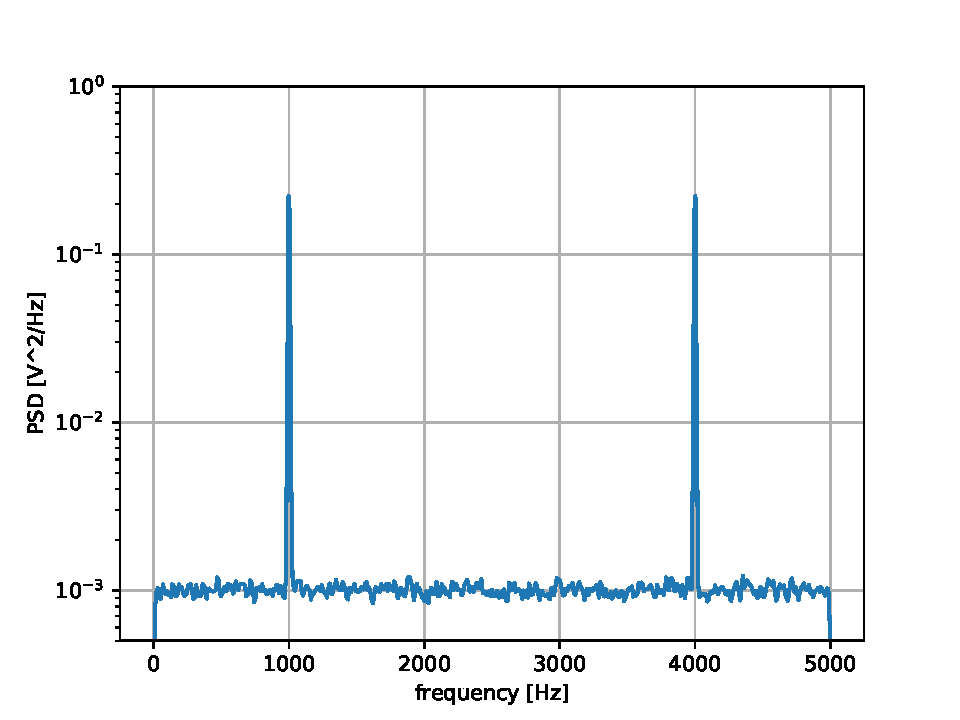
\includegraphics[width=0.9\textwidth]{../figures/pwelch_1k_4k_10k}
					\vspace*{-5pt}
					\caption{Densidad espectral de potencia para la suma dos senos de 1kHz y 4kHz muestreados a 10ksps}
				\end{subfigure}%
				\hspace*{10pt}
				\begin{subfigure}[t]{0.5\textwidth}
					\centering
					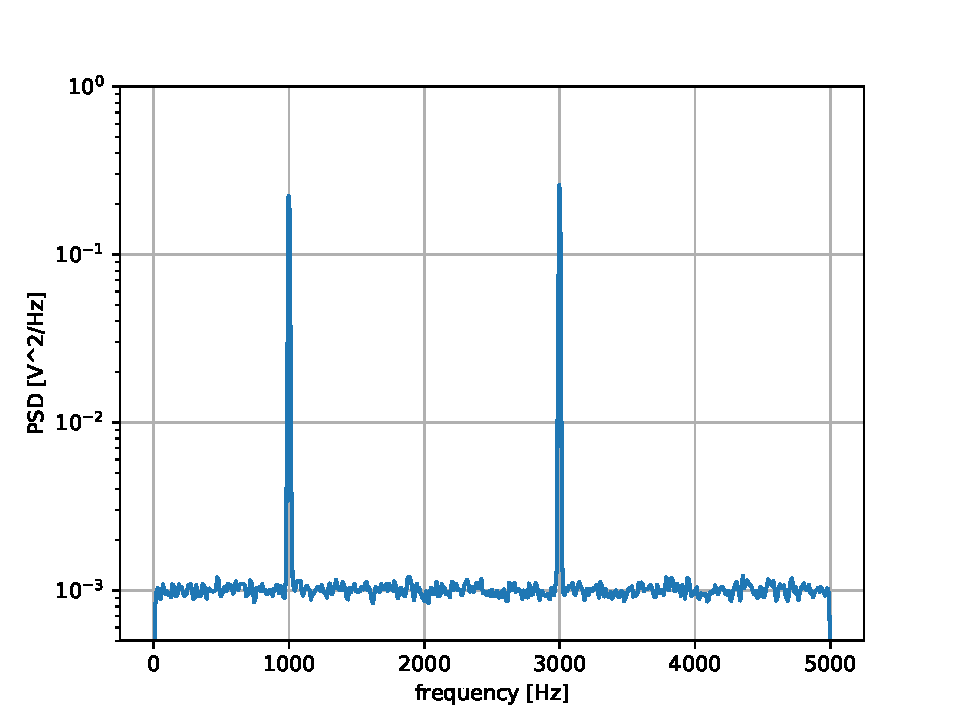
\includegraphics[width=0.9\textwidth]{../figures/pwelch_1k_7k_10k}
					\vspace*{-5pt}
					\caption{Densidad espectral de potencia para la suma dos senos de 1kHz y 7kHz submuestreados a 10ksps}
				\end{subfigure}
				\label{fig: aliasing}
			\end{figure}
		}
	\end{columns}
\end{frame}
\begin{frame}{Introducción al procesamiento de señal. Cuantización}
	\begin{block}{\centering \footnotesize Digitalización}
		%\centering
		Proceso mediante el cual, una señal $x(n)$ discreta en tiempo y continua en valores pasa a una señal digital $x_q(n)$ discreta en tiempo y en valores.
	\end{block}
	\begin{columns}
		\column[]{0.45\textwidth}
		{
			\begin{figure}[ht!]
				\centering
				\resizebox{\textwidth}{!}{
					\begin{tikzpicture}
					\tikzstyle{stealth} = [-stealth, thick]
					\tikzstyle{invisible} = [outer sep=0,inner sep=0,minimum size=0]
					\tikzstyle{circle} = [shape=circle, minimum size=0.5cm, draw=black!55]
					\tikzstyle{line} = [draw, very thick, red]
					\draw (-0.5,1)node[left,font=\tiny] {} -- (10.5,1);
					\draw (-0.5,0.7142)node[left,font=\tiny] {} -- (10.5,0.7142);
					\draw (-0.5,0.4285)node[left,font=\tiny] {} -- (10.5,0.4285);
					\draw (-0.5,0.1428)node[left,font=\tiny] {} -- (10.5,0.1428);
					\draw (-0.5,-0.1428)node[left,font=\tiny] {} -- (10.5,-0.1428);
					\draw (-0.5,-0.4285)node[left,font=\tiny] {} -- (10.5,-0.4285);
					\draw (-0.5,-0.7142)node[left,font=\tiny] {} -- (10.5,-0.7142);
					\draw (-0.5,-1)node[left,font=\tiny] {$y=-1$} -- (10.5,-1);
					\foreach \x in {0,0.1,0.2,0.3,0.4,0.5,0.6,0.7,0.8,0.9,1}
					{
						\draw (\x*10,-1.5)node [below,font=\tiny,] {\x } -- (\x*10,1.5) ;
					}
					\draw[ultra thick, ] (0,0) node (v5) {} sin (2.5,1) node (v7) {};
					\draw[ultra thick, ] (2.5,1) cos (5,0) node (v9) {};
					\draw[ultra thick, ] (5,0) sin (7.5,-1) node (v11) {};
					\draw[ultra thick, ] (7.5,-1) cos (10,0) node (v13) {};
					
					\node [invisible] (v1) at (-0.5,-1.5) {};
					\node [invisible] (v2) at (-0.5,2) {amplitud};
					\node [invisible] (v3) at (11,-1.5) {tiempo};
					\draw [stealth] (v1) edge (v2);
					\draw [stealth] (v1) edge (v3);
					\node [circle] (v4) at (0,0.1428) {};
					\node [circle] (v6) at (1,0.7142) {};
					\node [circle] (v8) at (2,1) {};
					\node [circle] (v10) at (3,1) {};
					\node [circle] (v12) at (4,0.7) {};
					\node [circle] (v14) at (5,0.1) {};
					\node [circle] at (6,-0.7) {};
					\node [circle] (v15) at (7,-1) {};
					\node [circle] at (8,-1) {};
					\node [circle] (v16) at (9,-0.7) {};
					\node [circle] (v17) at (10,0) {};
					\draw [line](0,0.1428) -- (1,0.1428) node [invisible] {} -- (1,0.7) -- 
					(2,0.7) node [invisible] {} -- (2,1) -- 
					(4,1) node [invisible] {} -- (4,0.7) -- 
					(5,0.7) node [invisible] {} -- (5,0.1) node [invisible] {} --
					(6,0.1) -- (6,-0.7) node [invisible] {} --
					(7,-0.7) node [invisible] {} -- (7,-1) -- 
					(9,-1) node [invisible] {} -- (9,-0.7) -- (10,-0.7) -- (10,-0.14);
					\end{tikzpicture}
				}      
				\caption{Esquema de la cuantización con 4 bits a 10 muestras por segundo, i.e., 8 valores posibles}
				\label{fig: cuantization_4bit}
			\end{figure}
		}
		\column[]{0.45\textwidth}
		{
			\begin{figure}[ht!]
				\centering
				\resizebox{\textwidth}{!}{
					\begin{tikzpicture}
					\tikzstyle{stealth} = [-stealth, thick]
					\tikzstyle{invisible} = [outer sep=0,inner sep=0,minimum size=0]
					\tikzstyle{circle} = [shape=circle, minimum size=0.5cm, draw=black!55]
					\tikzstyle{line} = [draw, very thick, red]
					
					\draw (0,0) node [invisible] (v1) {} --
					(4,0) node [invisible] {} --
					(4,4) node [invisible] {} --
					(0,4) node [invisible] {} --
					(0,0) node [invisible] {};
					\foreach \x in {0,0.25,0.5,0.75,1}
					{
						\draw (\x*4,-0.1)node [below,font=\tiny,] {\x } -- (\x*4,0.1) ;
					}
					\foreach \x in {0.125,0.375,0.625,0.875,1}
					{
						\draw (\x*4,-0.1)node [below,font=\tiny,] {} -- (\x*4,0.1);
					}
					\foreach \c [count=\x from 0] in {{000},{001},{010},{011},{100},{101},{110},{111}}
					{
						\draw (-0.1,\x*0.5)node [anchor=east,font=\tiny,] {\c} -- (0.1,\x*0.5);
					}
					%\node at (0,\x) {\c};	
					\draw [line](v1) -- (0.25,0) node [invisible] {} -- 
					(0.25,0.5) node [invisible] {} -- 
					(0.75,0.5) node [invisible] {} -- 
					(0.75,1) node [invisible] {} -- 
					(1.25,1) node [invisible] {} -- 
					(1.25,1.5) node [invisible] {} -- 
					(1.75,1.5) node [invisible] {} -- 
					(1.75,2) node [invisible] {} -- 
					(2.25,2) node [invisible] {} -- 
					(2.25,2.5) node [invisible] {} -- 
					(2.75,2.5) node [invisible] {} -- 
					(2.75,3) node [invisible] {} -- 
					(3.25,3) node [invisible] {} -- 
					(3.25,3.5) node [invisible] {} -- 
					(4,3.5) node [invisible] {};
					\node [invisible] at (2.0187,-1) {$(V_{in}-V_{RefLo})/E_{FSR}$};
					\node [invisible, rotate=90] at (-0.8509,1.9232) {$ADC_{code}$};
					\draw [dashed](0,2) node [invisible] {} -- (2,2) node [invisible] {} -- (2,0) node [invisible] {};
					\draw [dashed](0,3.5) node [invisible] {} -- (3.5,3.5) node [invisible] {} -- (3.5,0) node [invisible] {};
					\draw [dashed](0.25,4) node [] {} -- (0.25,-0.25) node [anchor=north] {\tiny LSB};
					\end{tikzpicture}
				}      
				\caption{Resolución del ADC}
				\label{fig: adc_resolution}
			\end{figure}
		}
	\end{columns}
\end{frame}
		\subsection{Redes LSTM}
			\begin{frame}{Redes recurrentes. Celdas LSTM}
	\begin{columns}
		\column[]{0.45\textwidth}
		{
			\begin{itemize}
				\item Redes \textbf{recurrentes} \arrowTikz{0} Las redes neuronales recurrentes son aquellas que retienen información de sus estados anteriores y ante los mismos estímulos de entrada no siempre producen las mismas salidas, debido al estado de la celda.
			\end{itemize}
		}
		\column[]{0.45\textwidth}
		{
			\begin{figure}[ht!]
				\centering
				\resizebox{0.9\textwidth}{!}{
					\begin{tikzpicture}
					\tikzstyle{box} = [draw,inner sep=7,minimum size=57,line 
					width=1, very thick, draw=black, fill=black!20, text width=60pt, text centered]
					\tikzstyle{stealth} = [-stealth, thick]
					\tikzstyle{invisible} = [outer sep=0,inner sep=0,minimum size=0]
					\tikzstyle{circle} = [shape=circle, minimum size=0.5cm, draw=black!55]
					\tikzstyle{line} = [draw, very thick, red]
					
					\begin{scope}
					\node [box] (v2) at (0,0) {Neurona tradicional};
					\node [circle, fill] (v1) at (0,2.5) {};
					\node [circle, fill] (v3) at (0,-2.5) {};
					\draw [stealth] (v1) edge node[anchor=east] {$x(t)$} (v2);
					\draw [stealth] (v2) edge node[anchor=east] {$y(t)$} (v3);
					\end{scope}
					\begin{scope}[shift={(3.5,0)}]
					\node [box] (v2_1) at (0,0) {Neurona recurrente};
					\node [circle, fill] (v1_1) at (0,2.5) {};
					\node [circle, fill] (v3_1) at (0,-2.5) {};
					\draw [stealth] (v1_1) edge node [anchor=east] {$x(t)$} (v2_1);
					\draw [stealth] (v2_1) edge node [anchor=east] {$y(t)$} (v3_1);
					\end{scope}
					
					\node [invisible, anchor=east] (v5) at (4.75,1.25) {};
					\draw [stealth, in =0, out=0] (v5) edge node[anchor=north west] {$h(t-1)$} (v2_1);
					\node [invisible] (v4) at (2.25,1.25) {};
					\node [] (v6) at (3.5,1.25) {};
					\draw [thick, in =180, out=180] (v2_1) edge (v4);
					\draw [thick] (v4) edge (v6);
					\draw [thick] (v6) edge (v5);
					\end{tikzpicture}
				}      
				\caption{Comparación de neuronas tradicionales con neuronas recurrentes}
				\label{fig: nn_vs_rnn}
			\end{figure}
		}
	\end{columns}
	\begin{itemize}
		\item Celdas LSTM (Long Short-Term Memory)
		\begin{itemize}
			\item \scriptsize{Propuestas por Sepp Hochreiter y Jürgen Schmidhuber en 1997.}
			\item \scriptsize{Evitan el problema de las dependencias a largo plazo.}
		\end{itemize}
	\end{itemize}
	\vspace*{-5pt}
	\begin{figure}[ht!]
		\centering
		\resizebox{0.8\textwidth}{!}{
			\begin{tikzpicture}
			\tikzstyle{box} = [draw,minimum size=15,line width=1, very thick, draw=black, fill=black!30, text centered]
			\tikzstyle{stealth} = [-stealth, thick]
			\tikzstyle{invisible} = [outer sep=0,inner sep=0,minimum size=0]
			\tikzstyle{circle} = [shape=ellipse, minimum size=15pt, draw=black!, text width=15pt, text centered]
			\tikzstyle{circle_op} = [shape=circle, minimum size=0.5cm, draw=black, very thick, fill=black!10]
			\tikzstyle{line} = [draw, very thick, red]
			\begin{scope}
			\node [circle] (v14) at (-2.25,-0.75) {$x_t$};
			\node [box] (v1) at (-1.5,0.5) {$\sigma$};
			\node [box] (v3) at (-0.5,0.5) {$\sigma$};
			\node [box] (v8) at (0.5,0.5) {$\tanh$};
			\node [box] (v6) at (1.5,0.5) {$\sigma$};
			\node [circle_op] (v2) at (-1.5,2.5) {x};
			\node [circle_op] (v4) at (0.5,1.5) {x};
			\node [circle_op] (v5) at (0.5,2.5) {\scriptsize$+$};
			\node [circle_op] (v7) at (2.5,1.25) {x};
			\node [ellipse, draw, very thick, fill=black!10] (v13) at (2.5,2) {$\tanh$};
			\draw [stealth] (v1) edge (v2);
			\draw [stealth,out=90,in=180] (v3) edge (v4);
			\draw [stealth] (v4) edge (v5);
			\draw [stealth,out=90,in=180] (v6) edge (v7);
			\node [invisible] (v11) at (-2,0) {};
			\node [invisible] (v10) at (-0.5,0) {};
			\node [invisible] (v9) at (0.5,0) {};
			\node [invisible] (v12) at (1,0) {};
			\draw [thick] (v8) edge (v4);
			\draw [thick,] (v9) edge (v8);
			\draw [thick] (v10) edge (v3);
			\draw [thick] (v11) edge (v12);
			\draw [thick,out=0,in=270] (v12) edge (v6);
			\draw [thick] (v7) edge (v13);
			\draw [thick] (v2) edge (v5);
			\draw [thick,out=90,in=180] (v14) edge (v11);
			\draw [thick,out=0,in=270] (v11) edge (v1);
			\node [invisible] (v22) at (-2.75,0) {};
			\node [invisible] (v21) at (-2.75,2.5) {};
			\node [invisible] (v17) at (4,2.5) {};
			\node [circle] (v19) at (3.5,4) {$h_t$};
			\node [invisible] (v16) at (4,0) {};
			\node [invisible] (v15) at (3,0) {};
			\draw [stealth] (v15) edge (v16);
			\draw [stealth] (v5) edge (v17);
			\node (v18) at (3.5,2.5) {};
			\draw [stealth] (v18) edge (v19);
			\node [invisible] (v20) at (3.5,0) {};
			\draw [thick] (v20) edge (v18);
			\draw [thick,out=270,in=180] (v7) edge (v15);
			\draw [thick] (v21) edge (v2);
			\draw [thick] (v22) edge (v11);
			\node [invisible] (v23) at (2.5,2.5) {};
			\draw [thick] (v13) edge (v23);
			\draw [rounded corners=2ex] (-2.75,3) rectangle (3.75,-0.25);
			\end{scope}
			\begin{scope}[shift={(6.75,0)}]
			\node [circle] (v14) at (-2.25,-0.75) {$x_{t+1}$};
			\node [box] (v1) at (-1.5,0.5) {$\sigma$};
			\node [box] (v3) at (-0.5,0.5) {$\sigma$};
			\node [box] (v8) at (0.5,0.5) {$\tanh$};
			\node [box] (v6) at (1.5,0.5) {$\sigma$};
			\node [circle_op] (v2) at (-1.5,2.5) {x};
			\node [circle_op] (v4) at (0.5,1.5) {x};
			\node [circle_op] (v5) at (0.5,2.5) {\scriptsize$+$};
			\node [circle_op] (v7) at (2.5,1.25) {x};
			\node [ellipse, draw, very thick, fill=black!10] (v13) at (2.5,2) {$\tanh$};
			\draw [stealth] (v1) edge (v2);
			\draw [stealth,out=90,in=180] (v3) edge (v4);
			\draw [stealth] (v4) edge (v5);
			\draw [stealth,out=90,in=180] (v6) edge (v7);
			\node [invisible] (v11) at (-2,0) {};
			\node [invisible] (v10) at (-0.5,0) {};
			\node [invisible] (v9) at (0.5,0) {};
			\node [invisible] (v12) at (1,0) {};
			\draw [thick] (v8) edge (v4);
			\draw [thick,] (v9) edge (v8);
			\draw [thick] (v10) edge (v3);
			\draw [thick] (v11) edge (v12);
			\draw [thick,out=0,in=270] (v12) edge (v6);
			\draw [thick] (v7) edge (v13);
			\draw [thick] (v2) edge (v5);
			\draw [thick,out=90,in=180] (v14) edge (v11);
			\draw [thick,out=0,in=270] (v11) edge (v1);
			\node [invisible] (v22) at (-2.75,0) {};
			\node [invisible] (v21) at (-2.75,2.5) {};
			\node [invisible] (v17) at (4,2.5) {};
			\node [circle] (v19) at (3.5,4) {$h_{t+1}$};
			\node [invisible] (v16) at (4,0) {};
			\node [invisible] (v15) at (3,0) {};
			\draw [stealth] (v15) edge (v16);
			\draw [stealth] (v5) edge (v17);
			\node (v18) at (3.5,2.5) {};
			\draw [stealth] (v18) edge (v19);
			\node [invisible] (v20) at (3.5,0) {};
			\draw [thick] (v20) edge (v18);
			\draw [thick,out=270,in=180] (v7) edge (v15);
			\draw [thick] (v21) edge (v2);
			\draw [thick] (v22) edge (v11);
			\node [invisible] (v23) at (2.5,2.5) {};
			\draw [thick] (v13) edge (v23);
			\draw [rounded corners=2ex,fill=black!60,opacity=0.8] (-2.75,3) rectangle (3.75,-0.25);
			\end{scope}
			\begin{scope}[shift={(-6.75,0)}]
			\node [circle] (v14) at (-2.25,-0.75) {$x_{t-1}$};
			\node [box] (v1) at (-1.5,0.5) {$\sigma$};
			\node [box] (v3) at (-0.5,0.5) {$\sigma$};
			\node [box] (v8) at (0.5,0.5) {$\tanh$};
			\node [box] (v6) at (1.5,0.5) {$\sigma$};
			\node [circle_op] (v2) at (-1.5,2.5) {x};
			\node [circle_op] (v4) at (0.5,1.5) {x};
			\node [circle_op] (v5) at (0.5,2.5) {\scriptsize$+$};
			\node [circle_op] (v7) at (2.5,1.25) {x};
			\node [ellipse, draw, very thick, fill=black!10] (v13) at (2.5,2) {$\tanh$};
			\draw [stealth] (v1) edge (v2);
			\draw [stealth,out=90,in=180] (v3) edge (v4);
			\draw [stealth] (v4) edge (v5);
			\draw [stealth,out=90,in=180] (v6) edge (v7);
			\node [invisible] (v11) at (-2,0) {};
			\node [invisible] (v10) at (-0.5,0) {};
			\node [invisible] (v9) at (0.5,0) {};
			\node [invisible] (v12) at (1,0) {};
			\draw [thick] (v8) edge (v4);
			\draw [thick,] (v9) edge (v8);
			\draw [thick] (v10) edge (v3);
			\draw [thick] (v11) edge (v12);
			\draw [thick,out=0,in=270] (v12) edge (v6);
			\draw [thick] (v7) edge (v13);
			\draw [thick] (v2) edge (v5);
			\draw [thick,out=90,in=180] (v14) edge (v11);
			\draw [thick,out=0,in=270] (v11) edge (v1);
			\node [invisible] (v22) at (-2.75,0) {};
			\node [invisible] (v21) at (-2.75,2.5) {};
			\node [invisible] (v17) at (4,2.5) {};
			\node [circle] (v19) at (3.5,4) {$h_{t-1}$};
			\node [invisible] (v16) at (4,0) {};
			\node [invisible] (v15) at (3,0) {};
			\draw [stealth] (v15) edge (v16);
			\draw [stealth] (v5) edge (v17);
			\node (v18) at (3.5,2.5) {};
			\draw [stealth] (v18) edge (v19);
			\node [invisible] (v20) at (3.5,0) {};
			\draw [thick] (v20) edge (v18);
			\draw [thick,out=270,in=180] (v7) edge (v15);
			\draw [thick] (v21) edge (v2);
			\draw [thick] (v22) edge (v11);
			\node [invisible] (v23) at (2.5,2.5) {};
			\draw [thick] (v13) edge (v23);
			\draw [rounded corners=2ex,fill=black!60,opacity=0.8] (-2.75,3) rectangle (3.75,-0.25);
			\end{scope}
			\end{tikzpicture}
		}
		\vspace*{-5pt}
		\caption{Celdas LSTM}
		\label{fig: lstm}
	\end{figure}
\end{frame}
		\subsection{Estado del arte}
			\begin{frame}[t]{Estado del Arte}
	\begin{table} [h!]
		\centering
		\resizebox{\textwidth}{!}{%
			\begin{tabular}{C{0.6\textwidth} C{0.4\textwidth}}
				\normalsize{\textbf{Algoritmos dominio público}} & \normalsize{\textbf{Algoritmos privativos}} \\ \bottomrule
			\end{tabular}
		}
	\end{table}
	\begin{columns}
		\begin{column}{0.6\textwidth}
			\centering
			\vspace*{-10pt}
			\begin{figure}[ht!]
				\centering
				\begin{subfigure}[t]{0.45\textwidth}
					\centering
					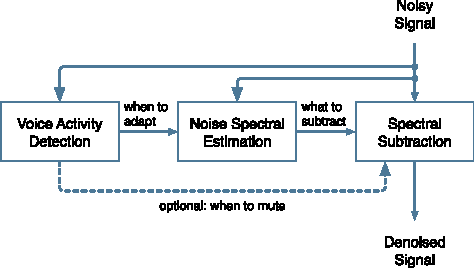
\includegraphics[width=0.9\textwidth]{../figures/rnn_structure.pdf}
					\caption{Estructura del algoritmo presentado por Jean-Marc Valin}
					\label{fig: rnn_structure}
				\end{subfigure}%
				\hspace*{10pt}
				\begin{subfigure}[t]{0.45\textwidth}
					\centering
					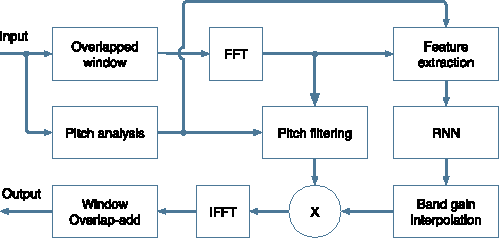
\includegraphics[width=0.9\textwidth]{../figures/rnn_block_diagram.pdf}
					\caption{Diagrama de bloques del eliminación de ruido en el dominio de la frecuencia}
					\label{fig: rnn_block_diagram}
				\end{subfigure}
				\begin{subfigure}[b]{0.65\textwidth}
					\centering
					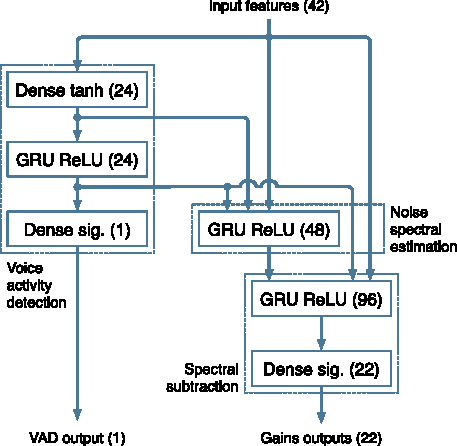
\includegraphics[width=0.9\textwidth]{../figures/rnn_nn.pdf}
					\caption{Red neuronal de RNNoise}
					\label{fig: rnn_nn}
				\end{subfigure}
			\end{figure}
		\end{column}
		\vrule{}
		\begin{column}[t]{0.4\textwidth}
			\vspace*{-100pt}
			\begin{itemize}
				\item \textbf{RTX Voice}
				\begin{itemize}
					\scriptsize
					\item Producto de NVIDIA
					\item \checkTikz{0.2}Gratuito
					\item \redcrossTikz{0.2}Plugins para algunas aplicaciones de chat por voz
					\item \redcrossTikz{0.2}Necesita una gráfica NVIDIA RTX
				\end{itemize}
				\item \textbf{Krisp}
				\begin{itemize}
					\scriptsize
					\item Producto de Krisp
					\item \redcrossTikz{0.2}De pago (gratuito hasta 120$\frac{min}{semana}$)
					\item \checkTikz{0.2}Funciona con el dispositivo de audio del sistema operativo, luego funciona con todo
					\item \checkTikz{0.2}No necesita hardware dedicado
				\end{itemize}
			\end{itemize}
		\end{column}
	\end{columns}
\end{frame}
	% DATA GATHERING
	\section{Obtención, procesado y almacenamiento de datos}
		\subsection{Datos de Audio}
			\begin{frame}[t]{Obtención, procesado y almacenamiento de datos. Pistas de Audio I}
	\begin{table} [h!]
		\centering
		\resizebox{\textwidth}{!}{%
			\begin{tabular}{C{0.5\textwidth} C{0.5\textwidth}}
				\normalsize{\textbf{Extracción del audios de videos de Youtube}} & \normalsize{\textbf{Generación sintética}} \\ \bottomrule
			\end{tabular}
		}
	\end{table}
	\begin{columns}
		\begin{column}{0.5\textwidth}
			\centering
			\vspace*{-10pt}
			\begin{itemize}
				\item \checkTikz{0.2}Gran cantidad fuente de información
				\item \redcrossTikz{0.2}Vídeos de todo tipo que pueden contener ruido
				\item \redcrossTikz{0.2}Una descarga masiva requiere una revisión de todos los audios obtenidos
			\end{itemize}
		\end{column}
		\vrule{}
		\begin{column}[t]{0.5\textwidth}
			\vspace*{-40pt}
			\begin{itemize}
				\item A partir de audios existentes
				\begin{itemize}
					\scriptsize
					\item \redcrossTikz{0.2}En audio no tiene sentido. Se usa en entorno de imágenes donde éstas se giran o se ordenan las columnas en orden inverso (espejo)
				\end{itemize}
				\item A partir de texto (Text to speech)
				\begin{itemize}
					\scriptsize
					\item \checkTikz{0.2}Fuente infinita
					\item \checkTikz{0.2}Conocimiento de lo que se dice (se genera a partir de texto)
					\item \redcrossTikz{0.2}Sintetizadores tradicionales generan voces metálicas
					\item \redcrossTikz{0.2}Sintetizadores basados en NN costosos de entrenar (Real Time Voice Cloning)
				\end{itemize}
			\end{itemize}
		\end{column}
	\end{columns}
\end{frame}
\begin{frame}[t]{Obtención, procesado y almacenamiento de datos. Pistas de Audio II}
	\begin{table} [h!]
		\centering
		\resizebox{\textwidth}{!}{%
			\begin{tabular}{C{\textwidth}}
				\normalsize{\textbf{Descarga masiva de audiolibros}}\\ \bottomrule
			\end{tabular}
		}
	\end{table}
	\begin{columns}
		\begin{column}{0.5\textwidth}
			Técnica de web scrapping:
			\begin{itemize}
				\item Exploración visual del sitio web.
				\item Análisis de la URL. En muchas ocasiones, parte de la información que el sitio web devuelve viene filtrada mediante una serie de filtros que se definen en la URL.
				\item Análisis del sitio web mediante herramientas de desarrollador. Consiste analizar el sitio web para encontrar dónde está la información que se quiere extraer y cómo viene en el código de la página. Para esto se usa un navegador web y se analiza el código mediante el inspector del navegador. Esta herramienta resalta cada una de las partes del código de la página web que se corresponden con las partes visuales de la misma.
				\item Extracción y almacenamiento de la información.
			\end{itemize}
		\end{column}
		\vrule{}
		\begin{column}[t]{0.5\textwidth}
			\vspace*{-100pt}
			\begin{figure}[ht!]
				\centering
				\resizebox{!}{0.65\textheight}{
					\begin{tikzpicture}
					\tikzstyle{box} = [draw,inner sep=7,minimum size=57,line 
					width=1, very thick, draw=black, fill=black!20, text width=120, text centered]
					\tikzstyle{invisible} = [outer sep=0,inner sep=0,minimum size=0]
					\tikzstyle{stealth} = [-stealth]
					
					\tikzstyle{decision} = [diamond, draw, fill=yellow!20, 
					text width=6em, text badly centered, node distance=3cm, inner sep=0pt]
					\tikzstyle{block} = [rectangle, draw, fill=gray!20, 
					text width=12em, text centered, rounded corners, minimum height=4em]
					\tikzstyle{small_block} = [circle, draw, fill=white!20, 
					text width=0em, text centered, rounded corners, minimum height=0em]    
					\tikzstyle{cloud} = [draw, ellipse,fill=red!20, node distance=3cm,
					minimum height=2em]
					
					\node [cloud] (v8) at (0,3.5) {\textbf{Start}};
					\node [block] (v3) at (0,1.5) {\vspace*{-0pt}\begin{itemize}
						\item lastPage=0 \vspace*{-0pt}
						\item increaseSleep=0 \vspace*{-0pt}
						\item page=1 \vspace*{-0pt}
						\item availablePage=True
						\end{itemize}};
					\node [block] (v2) at (0,-1) {Update URL\\ GET URL};
					\node [block] (v4) at (0,-3) {Sleep[random(0.5,1) + increaseSlepp]};
					\node [block] (v5) at (0,-5) {Parse lastPageNode};
					\node [decision] (v6) at (0,-8) {lastPageNode == Null?};
					\node [block] (v1) at (-3.5,-10) {increaseSleep+=1};
					\node [block] (v7) at (3.5,-10) {increaseSleep=0};
					\draw [stealth,out=180,in=180] (v1) edge (v2);
					\draw [stealth] (v3) edge (v2);
					\draw [stealth] (v2) edge (v4);
					\draw [stealth] (v4) edge (v5);
					\draw [stealth] (v5) edge (v6);
					\draw [stealth,out=180,in=90] (v6) edge node[anchor=east]{YES} (v1);
					\draw [stealth,out=0,in=90] (v6) edge node[anchor=west]{NO} (v7);
					\draw [stealth] (v8) edge (v3);
					\node [decision] (v9) at (3.5,-13) {lastPage == 0?};
					\node [block] (v10) at (-1,-14.5) {Update lastPage val(lastPageNode)};
					\draw [stealth,out=180,in=90] (v9) edge node [anchor=south east]{YES} (v10);
					\node [block] (v13) at (3.5,-16.5) {Parse information for every book in the query};
					\node [block] (v12) at (-1,-21) {page+=1};
					\node [decision] (v11) at (3.5,-19.5) {page == lastPage?};
					\draw [stealth,out=180,in=90] (v11) edge  node [anchor=south east]{NO} (v12);
					\draw [stealth,out=180,in=180] (v12) edge (v2);
					\draw [stealth] (v9) edge node [anchor=south east]{NO} (v13);
					\draw [stealth] (v7) edge (v9);
					\draw [stealth] (v13) edge (v11);
					\draw [stealth,out=270,in=180] (v10) edge (v13);
					\node [cloud] (v14) at (5.5,-21) {\textbf{end}};
					\draw [stealth,out=0,in=90] (v11) edge node[anchor=west]{YES} (v14);
					\end{tikzpicture}
				}      
				\caption{Diagrama de flujo para el scraper de LibriVox}
				\label{fig: librivox_scraper_flowchart}
			\end{figure}
		\end{column}
	\end{columns}
\end{frame}
		\subsection{Datos de Ruido}
			\begin{frame}{Obtención, procesado y almacenamiento de datos. Pistas de Ruido}
	Descarga de videos con ruido a partir de YouTube y extracción de audio
	\begin{itemize}
		\item Ruido de ciudad
		\item Ruido de lluvia
		\item Ruido de murmullo
		\item Librería \textit{youtube\_dl}
		\item Almacenamiento en base de datos de toda la información de las pistas
	\end{itemize}
\end{frame}
	% EDA
	\section{Análisis exploratorio de datos}
		\subsection{Análisis de integridad}
			\begin{frame}{Análisis exploratorio de datos. Integridad}
	\begin{columns}
			\hspace*{-30pt}
		\begin{column}{0.7\textwidth}
			\begin{table} [ht!]
				\renewcommand{\arraystretch}{0.2}
				\centering
				\resizebox{0.9\columnwidth}{!}{%
					\tiny
					\begin{tabular}{L{0.25\columnwidth} C{0.1\columnwidth} L{0.8\columnwidth}}
						\toprule
						\textbf{Nombre} & \textbf{Tipo de dato} & \textbf{Descripción}\\ \midrule
						id & int & Identificador de la pista de audio \\ \midrule
						book\_name\_dummy & text & Nombre del libro con caracteres ASCII reducidos \\ \midrule
						book\_name & text & Nombre completo del libro \\ \midrule
						book\_author & text & Autor del libro \\ \midrule
						book\_url & text & URL de descarga del libro \\ \midrule
						book\_language & text & Lenguaje del libro \\ \midrule
						book\_path & text & Dirección de almacenamiento del libro comprimido \\ \midrule
						book\_n\_tracks & int & Número de pistas del libro \\ \midrule
						track\_name & text & Nombre de la pista de audio \\ \midrule
						track\_path & text & Directorio de almacenamiento de la pista de audio \\ \midrule
						track\_channels & int & Número de canales de la pista de audio \\ \midrule
						track\_sample\_rate & int & Tasa de muestreo de la pista de audio \\ \midrule
						track\_duration & real & Duración de la pista de audio \\ \midrule
						track\_status & text & Estado del archivo (OK\arrowTikz{0}descargado, DELETED\arrowTikz{0}eliminado) \\ \midrule
						track\_insert\_datetime & int & Fecha y hora de inserción del registro \\ \bottomrule
					\end{tabular}
				}
				\caption{Columnas de la tabla pista de los audiolibros}\label{tab: audio_book_table}
			\end{table}
		\end{column}
		\hspace*{-30pt}
		\begin{column}[t]{0.3\textwidth}
			\vspace*{-60pt}
			\begin{table} [b!]
				\centering
				\resizebox{1.3\textwidth}{!}{%
					\begin{tabular}{L{2cm} C{2cm} C{3cm}}
						\toprule
						\textbf{Tipo de pista} & \textbf{Duración [horas]} & \textbf{Tasas de muestreo [$\frac{muestras}{segundo}$]}\\ \midrule
						Audiolibros & 707.70 (555.73) & [22050]\\ \midrule
						Ruido & 52.91 & [44100, 48000]\\ \bottomrule
					\end{tabular}
				}
				\vspace*{3pt}
				\caption{Duración total de todas las pistas}\label{tab: duration}
			\end{table}
		\end{column}
	\end{columns}
	\vspace*{-10pt}
	\begin{table} [h!]
		\centering
		\resizebox{\textwidth}{!}{%
			\begin{tabular}{L{0.6cm} L{7cm} L{10cm}}
				\toprule
				\textbf{id} & \textbf{book\_name} & \textbf{track\_name}\\ \midrule
				1351 & Antología de Cuentos Fantásticos & antologiacuentosfantasticos\_01\_various\_64kb.mp3 \\ \midrule
				3410 & Coppelius (1ra Parte) (in  Antología de Cuentos Fantásticos ) & antologiacuentosfantasticos\_01\_various\_64kb.mp3 \\ \midrule
				3935 & De lo que aconteció a un deán de Santiago con don Illan el mágico, que moraba en Toledo (in  Antología de Cuentos Fantásticos ) & antologiacuentosfantasticos\_01\_various\_64kb.mp3 \\ \midrule
			\end{tabular}
		}
		\caption{Ejemplo de registros repetidos}\label{tab: repeat_registers}
	\end{table}
\end{frame}
		\subsection{Análisis de los datos de audio}
			\chapter{Análisis exploratorio de datos}\label{ch: eda}
Para el análisis exploratorio de datos, en primer lugar, se van a analizar la dimensión y las propiedades de datos a través una serie de querys a la base de datos donde se han almacenado los metadatos del dataset.

Los metadatos han sido divididos en dos tablas en función del lugar a dónde pertenecen. La primera tabla hace referencia a las pistas de los audiolibros y la segunda a los ruidos. La tabla \ref{tab: audio_book_table} presenta la columnas que contiene la tabla de las pistas de audio y la \ref{tab: noise_table} los metadatos de las pistas de ruido.

\begin{table} [ht!]
	\centering
	\resizebox{\columnwidth}{!}{%
		\begin{tabular}{L{5cm} C{3cm} L{15cm}}
			\toprule
			\textbf{Nombre} & \textbf{Tipo de dato} & \textbf{Descripción}\\ \midrule
			id & int & Identificador de la pista de audio \\ \midrule
			book\_name\_dummy & text & Nombre del libro con caracteres \acrshort{ASCII} reducidos \\ \midrule
			book\_name & text & Nombre completo del libro \\ \midrule
			book\_author & text & Autor del libro \\ \midrule
			book\_url & text & \gls{URL} de descarga del libro \\ \midrule
			book\_language & text & Lenguaje del libro \\ \midrule
			book\_path & text & Dirección de almacenamiento del libro comprimido \\ \midrule
			book\_n\_tracks & int & Número de pistas del libro \\ \midrule
			track\_name & text & Nombre de la pista de audio \\ \midrule
			track\_path & text & Directorio de almacenamiento de la pista de audio \\ \midrule
			track\_channels & int & Número de canales de la pista de audio \\ \midrule
			track\_sample\_rate & int & Tasa de muestreo de la pista de audio \\ \midrule
			track\_duration & real & Duración de la pista de audio \\ \midrule
			track\_status & text & Estado del archivo (OK\arrowTikz{0}descargado, DELETED\arrowTikz{0}eliminado) \\ \midrule
			track\_insert\_datetime & int & Fecha y hora de inserción del registro \\ \bottomrule
		\end{tabular}
	}
	\vspace*{3pt}
	\caption{Columnas de la tabla pista de los audiolibros}\label{tab: audio_book_table}
\end{table}

\begin{table} [ht!]
	\centering
	\resizebox{\columnwidth}{!}{%
		\begin{tabular}{L{5cm} C{3cm} L{15cm}}
			\toprule
			\textbf{Nombre} & \textbf{Tipo de dato} & \textbf{Descripción}\\ \midrule
			id & int & Identificador de la pista de ruido \\ \midrule
			name & text & Nombre del ruido que coincide con el nombre del archivo \acrshort{ASCII} reducidos \\ \midrule
			url & text & \gls{URL} de descarga del video que contiene el ruido \\ \midrule
			path & text & Dirección de almacenamiento de la pista de ruido \\ \midrule
			channels & int & Número de canales de la pista de ruido \\ \midrule
			sample\_rate & int & Tasa de muestreo de la pista de ruido \\ \midrule
			duration & real & Duración de la pista de ruido \\ \midrule
			status & text & Estado del archivo (OK\arrowTikz{0}descargado, DELETED\arrowTikz{0}eliminado) \\ \midrule
			insert\_datetime & int & Fecha y hora de inserción del registro \\ \bottomrule
		\end{tabular}
	}
	\vspace*{3pt}
	\caption{Columnas de la tabla con los metadatos de las pista de ruido}\label{tab: noise_table}
\end{table}

A partir de las tablas se pueden sacar datos que den una idea de la dimensión del problema y si los datos son compatibles entre ellos o no. Dos pistas de audio pueden ser no compatibles porque el algoritmo se diseña para una tasa de muestreo estática y, las pistas de audio o ruido, no tienen por qué tener tasas de muestreo que sean múltiplos y divisores comunes de la del modelo. En primer lugar se pueden ver la duración total de las pista de audiolibros y de ruido, para ello simplemente se lanza una query \textbf{agregando por el campo duración} con la función \textbf{SUM} como muestra la tabla \ref{tab: duration}.
\begin{table} [h!]
	\centering
	\resizebox{!}{!}{%
		\begin{tabular}{L{3cm} C{3cm} C{3cm}}
			\toprule
			\textbf{Tipo de pista} & \textbf{Duración [horas]} & \textbf{Tasas de muestreo [$\frac{muestras}{segundo}$]}\\ \midrule
			Audiolibros & 707.70 & [22050]\\ \midrule
			Ruido & 52.91 & [44100, 48000]\\ \bottomrule
		\end{tabular}
	}
	\vspace*{3pt}
	\caption{Duración total de todas las pistas}\label{tab: duration}
\end{table}

Otra métrica interesante es, como se comentó anteriormente, la compatibilidad de tasas de muestreo. Para ello se \textbf{agrega por el campo tasa de muestreo} con la función \textbf{DISTINCT}. El resultado se encuentra en la tabla \ref{tab: duration}.

A parte de obtener métricas, se pueden analizar la consistencia de los datos. Por ejemplo, se podría analizar si existen algunas pista de audio que se encuentren en varios libros. Esto se daría si la plataforma de almacenamiento metiera varios libros en una misma \gls{URL} de descarga. En \ref{lst: repeat_track} se puede ver el código que implementa la query. El resultado de esta query es que hay \textbf{162} registros que se encuentran, como mínimo, dos veces.

\begin{lstlisting}[style=SQL,basicstyle=\tiny\ttfamily, caption={Query para obtener las pistas repetidas en varios libros},captionpos=b, label={lst: repeat_track}]
SELECT track_name, COUNT(*) AS c
FROM audio_books_tracks
GROUP BY track_name
HAVING c > 1
ORDER BY c DESC
\end{lstlisting}

Como la query da resultados distintos de \textbf{NULL}, hay pistas de audiolibros que se han contado varias veces falseando las estadísticas. Realizando una query con alguno de los resultados se confirma que existen pistas que se encuentran en varios libros y, por tanto, son registros repetidos. En la tabla \ref{tab: repeat_registers} se puede ver una de las pistas que se encuentra repetida. Con este tipo de queries se puede ver que de los \textbf{4227} registros, únicos son \textbf{2802}.
\begin{table} [h!]
	\centering
	\resizebox{\textwidth}{!}{%
		\begin{tabular}{L{0.6cm} L{7cm} L{10cm}}
			\toprule
			\textbf{id} & \textbf{book\_name} & \textbf{track\_name}\\ \midrule
			1351 & Antología de Cuentos Fantásticos & antologiacuentosfantasticos\_01\_various\_64kb.mp3 \\ \midrule
			3410 & Coppelius (1ra Parte) (in  Antología de Cuentos Fantásticos ) & antologiacuentosfantasticos\_01\_various\_64kb.mp3 \\ \midrule
			3935 & De lo que aconteció a un deán de Santiago con don Illan el mágico, que moraba en Toledo (in  Antología de Cuentos Fantásticos ) & antologiacuentosfantasticos\_01\_various\_64kb.mp3 \\ \midrule
		\end{tabular}
	}
	\vspace*{3pt}
	\caption{Ejemplo de registros repetidos}\label{tab: repeat_registers}
\end{table}





	% MODEL DESIGN
	\section{Diseño e implementación de modelos}
		\subsection{Pre-procesado de datos}
			\begin{frame}{Diseño e implementación de modelos.\newline Preparación de los datos I}
	\begin{figure}[ht!]
		\centering
		\resizebox{\textwidth}{!}{
			\begin{tikzpicture}
			\tikzstyle{box} = [draw,inner sep=7,minimum size=57,line 
			width=1, very thick, draw=black, fill=black!20, text width=100, text centered]
			\tikzstyle{invisible} = [outer sep=0,inner sep=0,minimum size=0]
			\tikzstyle{stealth} = [-stealth, very thick]
			\begin{scope}[shift={(0.5,0)}]		
			\begin{scope}[shift={(-3.5,3.1)}, scale=0.5]
			\node [invisible] at (-1.2,1.7) {$FFT_n$};
			\draw (-3,0.5) node [invisible] {} -- (-2.8,0.3) node [invisible] {} -- (-2.6,0.2) node [invisible] {} -- (-2.4,0.8) node [invisible] {} -- (-2.2,0.2) node [invisible] {} -- (-2,0.3) node [invisible] {} -- (-1.9,0.2) node [invisible] {} -- (-1.8,0.4) node [invisible] {} -- (-1.7,0.2) node [invisible] {} -- (-1.6,1.4) node [invisible] {} -- (-1.5,0.2) node [invisible] {} -- (-1.3,0.3) node [invisible] (v4) {};
			\node [invisible] (v2) at (-3,1.6) {};
			\node [invisible] (v1) at (-3,-0.4) {};
			\node [invisible] (v3) at (0.6,-0.4) {};
			\draw [stealth] (v1) edge (v2);
			\draw [stealth] (v1) edge (v3);
			\draw [stealth](v4);
			\draw (v4) -- (-1.2,0.2) node [invisible] {} -- (-1.1,0.4) node [invisible] {} -- (-1,0.2) node [invisible] {} -- (-0.8,0.8) node [invisible] {} -- (-0.7,0.2) node [invisible] {} -- (-0.5,0.3) node [invisible] {} -- (-0.4,0.2) node [invisible] {} -- (-0.2,0.3) node [invisible] {} -- (-0.1,0.2) node [invisible] {} -- (0.1,1.1) node [invisible] {} -- (0.3,0.2) node [invisible] {};
			\end{scope}
			\begin{scope}[shift={(-3.1,1.8)}, scale=0.5]
			\node [invisible] at (-1.2,1.7) {$FFT_{n-1}$};
			\draw (-3,0.5) node [invisible] {} -- (-2.8,0.3) node [invisible] {} -- (-2.6,0.2) node [invisible] {} -- (-2.4,0.8) node [invisible] {} -- (-2.2,0.2) node [invisible] {} -- (-2,0.3) node [invisible] {} -- (-1.9,0.2) node [invisible] {} -- (-1.8,0.4) node [invisible] {} -- (-1.7,0.2) node [invisible] {} -- (-1.6,1.4) node [invisible] {} -- (-1.5,0.2) node [invisible] {} -- (-1.3,0.3) node [invisible] (v4) {};
			\node [invisible] (v2) at (-3,1.6) {};
			\node [invisible] (v1) at (-3,-0.4) {};
			\node [invisible] (v3) at (0.6,-0.4) {};
			\draw [stealth] (v1) edge (v2);
			\draw [stealth] (v1) edge (v3);
			\draw [stealth](v4);
			\draw (v4) -- (-1.2,0.2) node [invisible] {} -- (-1.1,0.4) node [invisible] {} -- (-1,0.2) node [invisible] {} -- (-0.8,0.8) node [invisible] {} -- (-0.7,0.2) node [invisible] {} -- (-0.5,0.3) node [invisible] {} -- (-0.4,0.2) node [invisible] {} -- (-0.2,0.3) node [invisible] {} -- (-0.1,0.2) node [invisible] {} -- (0.1,1.1) node [invisible] {} -- (0.3,0.2) node [invisible] {};
			\end{scope}
			\begin{scope}[shift={(-1.5,-0.9)}, scale=0.5]
			\node [invisible] at (-1.2,1.7) {$FFT_2$};
			\draw (-3,0.5) node [invisible] {} -- (-2.8,0.3) node [invisible] {} -- (-2.6,0.2) node [invisible] {} -- (-2.4,0.8) node [invisible] {} -- (-2.2,0.2) node [invisible] {} -- (-2,0.3) node [invisible] {} -- (-1.9,0.2) node [invisible] {} -- (-1.8,0.4) node [invisible] {} -- (-1.7,0.2) node [invisible] {} -- (-1.6,1.4) node [invisible] {} -- (-1.5,0.2) node [invisible] {} -- (-1.3,0.3) node [invisible] (v4) {};
			\node [invisible] (v2) at (-3,1.6) {};
			\node [invisible] (v1) at (-3,-0.4) {};
			\node [invisible] (v3) at (0.6,-0.4) {};
			\draw [stealth] (v1) edge (v2);
			\draw [stealth] (v1) edge (v3);
			\draw [stealth](v4);
			\draw (v4) -- (-1.2,0.2) node [invisible] {} -- (-1.1,0.4) node [invisible] {} -- (-1,0.2) node [invisible] {} -- (-0.8,0.8) node [invisible] {} -- (-0.7,0.2) node [invisible] {} -- (-0.5,0.3) node [invisible] {} -- (-0.4,0.2) node [invisible] {} -- (-0.2,0.3) node [invisible] {} -- (-0.1,0.2) node [invisible] {} -- (0.1,1.1) node [invisible] {} -- (0.3,0.2) node [invisible] {};
			\end{scope}
			\begin{scope}[shift={(-1.1,-2.2)}, scale=0.5]
			\node [invisible] at (-1.2,1.7) {$FFT_1$};
			\draw (-3,0.5) node [invisible] {} -- (-2.8,0.3) node [invisible] {} -- (-2.6,0.2) node [invisible] {} -- (-2.4,0.8) node [invisible] {} -- (-2.2,0.2) node [invisible] {} -- (-2,0.3) node [invisible] {} -- (-1.9,0.2) node [invisible] {} -- (-1.8,0.4) node [invisible] {} -- (-1.7,0.2) node [invisible] {} -- (-1.6,1.4) node [invisible] {} -- (-1.5,0.2) node [invisible] {} -- (-1.3,0.3) node [invisible] (v4) {};
			\node [invisible] (v2) at (-3,1.6) {};
			\node [invisible] (v1) at (-3,-0.4) {};
			\node [invisible] (v3) at (0.6,-0.4) {};
			\draw [stealth] (v1) edge (v2);
			\draw [stealth] (v1) edge (v3);
			\draw [stealth](v4);
			\draw (v4) -- (-1.2,0.2) node [invisible] {} -- (-1.1,0.4) node [invisible] {} -- (-1,0.2) node [invisible] {} -- (-0.8,0.8) node [invisible] {} -- (-0.7,0.2) node [invisible] {} -- (-0.5,0.3) node [invisible] {} -- (-0.4,0.2) node [invisible] {} -- (-0.2,0.3) node [invisible] {} -- (-0.1,0.2) node [invisible] {} -- (0.1,1.1) node [invisible] {} -- (0.3,0.2) node [invisible] {};
			\end{scope}
			\node [circle, fill] at (-3.6,1.2) {};
			\node [circle, fill] at (-3.2,0.8) {};
			\node [circle, fill] at (-2.8,0.4) {};
			\draw [dashed, thick] (-5.5,6) node [invisible] (v5) {} -- (-5.5,-3.5) -- (-0.5,-3.5) -- (-0.5,6) -- (v5);
			\node [invisible] (v6) at (-0.5,0.75) {};
			\end{scope}
			
			\begin{scope}[shift={(10.5,0)}]		
			\begin{scope}[shift={(-1.2,3.1)}, scale=0.5]
			\node [invisible] at (-1.2,1.7) {$FFT_n$};
			\draw (-3,0.5) node [invisible] {} -- (-2.8,0.3) node [invisible] {} -- (-2.6,0.2) node [invisible] {} -- (-2.4,0.8) node [invisible] {} -- (-2.2,0.2) node [invisible] {} -- (-2,0.3) node [invisible] {} -- (-1.9,0.2) node [invisible] {} -- (-1.8,0.4) node [invisible] {} -- (-1.7,0.2) node [invisible] {} -- (-1.6,1.4) node [invisible] {} -- (-1.5,0.2) node [invisible] {} -- (-1.3,0.3) node [invisible] (v4) {};
			\node [invisible] (v2) at (-3,1.6) {};
			\node [invisible] (v1) at (-3,-0.4) {};
			\node [invisible] (v3) at (0.6,-0.4) {};
			\draw [stealth] (v1) edge (v2);
			\draw [stealth] (v1) edge (v3);
			\draw [stealth](v4);
			\draw (v4) -- (-1.2,0.2) node [invisible] {} -- (-1.1,0.4) node [invisible] {} -- (-1,0.2) node [invisible] {} -- (-0.8,0.8) node [invisible] {} -- (-0.7,0.2) node [invisible] {} -- (-0.5,0.3) node [invisible] {} -- (-0.4,0.2) node [invisible] {} -- (-0.2,0.3) node [invisible] {} -- (-0.1,0.2) node [invisible] {} -- (0.1,1.1) node [invisible] {} -- (0.3,0.2) node [invisible] {};
			\end{scope}
			\begin{scope}[shift={(-1.7,1.8)}, scale=0.5]
			\node [invisible] at (-1.2,1.7) {$FFT_{n-1}$};
			\draw (-3,0.5) node [invisible] {} -- (-2.8,0.3) node [invisible] {} -- (-2.6,0.2) node [invisible] {} -- (-2.4,0.8) node [invisible] {} -- (-2.2,0.2) node [invisible] {} -- (-2,0.3) node [invisible] {} -- (-1.9,0.2) node [invisible] {} -- (-1.8,0.4) node [invisible] {} -- (-1.7,0.2) node [invisible] {} -- (-1.6,1.4) node [invisible] {} -- (-1.5,0.2) node [invisible] {} -- (-1.3,0.3) node [invisible] (v4) {};
			\node [invisible] (v2) at (-3,1.6) {};
			\node [invisible] (v1) at (-3,-0.4) {};
			\node [invisible] (v3) at (0.6,-0.4) {};
			\draw [stealth] (v1) edge (v2);
			\draw [stealth] (v1) edge (v3);
			\draw [stealth](v4);
			\draw (v4) -- (-1.2,0.2) node [invisible] {} -- (-1.1,0.4) node [invisible] {} -- (-1,0.2) node [invisible] {} -- (-0.8,0.8) node [invisible] {} -- (-0.7,0.2) node [invisible] {} -- (-0.5,0.3) node [invisible] {} -- (-0.4,0.2) node [invisible] {} -- (-0.2,0.3) node [invisible] {} -- (-0.1,0.2) node [invisible] {} -- (0.1,1.1) node [invisible] {} -- (0.3,0.2) node [invisible] {};
			\end{scope}
			\begin{scope}[shift={(-3.2,-0.9)}, scale=0.5]
			\node [invisible] at (-1.2,1.7) {$FFT_2$};
			\draw (-3,0.5) node [invisible] {} -- (-2.8,0.3) node [invisible] {} -- (-2.6,0.2) node [invisible] {} -- (-2.4,0.8) node [invisible] {} -- (-2.2,0.2) node [invisible] {} -- (-2,0.3) node [invisible] {} -- (-1.9,0.2) node [invisible] {} -- (-1.8,0.4) node [invisible] {} -- (-1.7,0.2) node [invisible] {} -- (-1.6,1.4) node [invisible] {} -- (-1.5,0.2) node [invisible] {} -- (-1.3,0.3) node [invisible] (v4) {};
			\node [invisible] (v2) at (-3,1.6) {};
			\node [invisible] (v1) at (-3,-0.4) {};
			\node [invisible] (v3) at (0.6,-0.4) {};
			\draw [stealth] (v1) edge (v2);
			\draw [stealth] (v1) edge (v3);
			\draw [stealth](v4);
			\draw (v4) -- (-1.2,0.2) node [invisible] {} -- (-1.1,0.4) node [invisible] {} -- (-1,0.2) node [invisible] {} -- (-0.8,0.8) node [invisible] {} -- (-0.7,0.2) node [invisible] {} -- (-0.5,0.3) node [invisible] {} -- (-0.4,0.2) node [invisible] {} -- (-0.2,0.3) node [invisible] {} -- (-0.1,0.2) node [invisible] {} -- (0.1,1.1) node [invisible] {} -- (0.3,0.2) node [invisible] {};
			\end{scope}
			\begin{scope}[shift={(-3.7,-2.2)}, scale=0.5]
			\node [invisible] at (-1.2,1.7) {$FFT_1$};
			\draw (-3,0.5) node [invisible] {} -- (-2.8,0.3) node [invisible] {} -- (-2.6,0.2) node [invisible] {} -- (-2.4,0.8) node [invisible] {} -- (-2.2,0.2) node [invisible] {} -- (-2,0.3) node [invisible] {} -- (-1.9,0.2) node [invisible] {} -- (-1.8,0.4) node [invisible] {} -- (-1.7,0.2) node [invisible] {} -- (-1.6,1.4) node [invisible] {} -- (-1.5,0.2) node [invisible] {} -- (-1.3,0.3) node [invisible] (v4) {};
			\node [invisible] (v2) at (-3,1.6) {};
			\node [invisible] (v1) at (-3,-0.4) {};
			\node [invisible] (v3) at (0.6,-0.4) {};
			\draw [stealth] (v1) edge (v2);
			\draw [stealth] (v1) edge (v3);
			\draw [stealth](v4);
			\draw (v4) -- (-1.2,0.2) node [invisible] {} -- (-1.1,0.4) node [invisible] {} -- (-1,0.2) node [invisible] {} -- (-0.8,0.8) node [invisible] {} -- (-0.7,0.2) node [invisible] {} -- (-0.5,0.3) node [invisible] {} -- (-0.4,0.2) node [invisible] {} -- (-0.2,0.3) node [invisible] {} -- (-0.1,0.2) node [invisible] {} -- (0.1,1.1) node [invisible] {} -- (0.3,0.2) node [invisible] {};
			\end{scope}
			\node [circle, fill] at (-2.8,1.2) {};
			\node [circle, fill] at (-3.2,0.8) {};
			\node [circle, fill] at (-3.6,0.4) {};
			\draw [dashed, thick] (-5.5,6) node [invisible] (v5) {} -- (-5.5,-3.5) -- (-0.5,-3.5) -- (-0.5,6) -- (v5);
			\node [invisible] (v8) at (-5.5,0.75) {};
			\end{scope}
			
			\node [box,text width=60] (v7) at (2.5,0.75) {Modelo};
			
			
			\node [invisible] at (-2.5,5.5) {Módulo de FFT con ruido};
			\node [invisible] at (7.5,5.5) {Módulo de FFT sin ruido};
			\draw [stealth] (v6) edge (v7);
			\draw [stealth] (v7) edge (v8);
			\node [box] (v9) at (-8.5,7) {$Tiempo\xrightarrow{FFT}Frecuencia$};
			\node [box] (v10) at (13.5,7) {$Frecuencia\xrightarrow{iFFT}Tiempo$};
			\node [invisible] (v11) at (-5,0.75) {};
			\node [invisible] (v12) at (10,0.75) {};
			\draw [stealth,out=0,in=180] (v9) edge node[anchor=south]{Fase} (v10);
			\draw [stealth,out=0,in=180] (v9) edge node[anchor=east]{Módulo}(v11);
			\draw [stealth,out=0,in=180] (v12) edge node[anchor=west]{Módulo}(v10);
			\end{tikzpicture}
		}      
		\caption{Esquema de las entradas y salidas de datos del modelo}
		\label{fig: model_schema}
	\end{figure}
\end{frame}
\begin{frame}{Diseño e implementación de modelos.\newline Preparación de los datos II}
	\begin{figure}[ht!]
		\centering
		\resizebox{\textwidth}{!}{
			\begin{tikzpicture}
			\tikzstyle{box} = [draw,inner sep=7,minimum size=57,line 
			width=1, very thick, draw=black, fill=black!20, text width=80, text centered]
			\tikzstyle{invisible} = [outer sep=0,inner sep=0,minimum size=0]
			\tikzstyle{stealth} = [-stealth, very thick]
			\begin{scope} [scale=0.1, shift={(-112.5,10)}]
			\draw [very thick] (-2,0.5) arc (0:-180:1.5);
			\draw [very thick] (-2,3.5) arc (0:180:1.5);
			\node [invisible] (v1) at (-5,3.5) {};
			\node [invisible] (v3) at (-2,3.5) {};
			\node [invisible] (v2) at (-5,0.5) {};
			\node [invisible] (v4) at (-2,0.5) {};
			\draw [very thick] (v1) edge (v2);
			\draw [very thick] (v3) edge (v4);
			\node [invisible] (v9) at (-5,3) {};
			\node [invisible] (v10) at (-4,3) {};
			\node [invisible] (v11) at (-5,2) {};
			\node [invisible] (v12) at (-4,2) {};
			\node [invisible] (v13) at (-5,1) {};
			\node [invisible] (v14) at (-4,1) {};
			\node [invisible] (v15) at (-2,1) {};
			\node [invisible] (v16) at (-3,1) {};
			\node [invisible] (v17) at (-2,2) {};
			\node [invisible] (v18) at (-3,2) {};
			\node [invisible] (v19) at (-2,3) {};
			\node [invisible] (v20) at (-3,3) {};
			\draw [very thick] (-1.5,0.5) arc (0:-180:2);
			\node [invisible] (v7) at (-3.5,-1.5) {};
			\node [invisible] (v8) at (-3.5,-2.5) {};
			\node [invisible] (v5) at (-5.5,-2.5) {};
			\node [invisible] (v6) at (-1.5,-2.5) {};
			\draw [very thick] (v5) edge (v6);
			\draw [very thick] (v7) edge (v8);
			\draw [very thick] (v9) edge (v10);
			\draw [very thick] (v11) edge (v12);
			\draw [very thick] (v13) edge (v14);
			\draw [very thick] (v15) edge (v16);
			\draw [very thick] (v17) edge (v18);
			\draw [very thick] (v19) edge (v20);
			\end{scope}
			\node [box] (v23) at (-3,1) {Adaptación de la tasa de muestreo a $11025 \frac{muestras}{segundo}$};
			\node [box] (v22) at (-8.1,1) {Analógico $\xrightarrow{}$ Digital};
			\node [invisible] (v21) at (-11,1) {};
			\node [box] (v24) at (2.5,1) {FFT de $1024~muestras$};
			\node [box, minimum size=40] (v30) at (8.5,2.5) {Módulo};
			\node [box, minimum size=40] (v31) at (8.5,-0.5) {Fase};
			\node [box] (v26) at (2.5,-4.5) {$mod\cdot e^{j\cdot fase}$};
			\node [box] (v27) at (-3,-4.5) {iFFT};
			\node [box] (v28) at (-8.1,-4.5) {Analógico $\xleftarrow{}$ Digital};
			\begin{scope}[scale=0.4, shift={(-35.6,-8.15)}, xscale=-1]
			\draw [rounded corners, very thick, fill] (-7,-2.6) node [invisible] (v25) {} -- (-7,-3.6) node [invisible] {} -- (-6.5,-3.5) node [invisible] {} -- (-5.5,-4.5) node [invisible] {} -- (-5.5,-1.5) node [invisible] {} -- (-6.5,-2.5) node [invisible] {} -- (v25);
			\draw [very thick] (-5.0603,-2.658) arc (19.9988:-20:1);
			\draw [very thick] (-4.5905,-2.487) arc (19.9994:-20:1.5);
			\draw [very thick] (-4.1206,-2.316) arc (19.9988:-20:2);
			\draw [very thick] (-3.6508,-2.1449) arc (20.0013:-20:2.5);
			\end{scope}
			\node [invisible] (v29) at (-11,-4.5) {};
			\node [box, minimum size=40] (v32) at (8.5,-5) {Red neuronal recurrente};
			\draw [stealth] (v21) edge node [anchor=south]{$x_{in}(t)$} (v22);
			\draw [stealth] (v22) edge node [anchor=south]{$x_{in}(n)$}(v23);
			\draw [stealth] (v23) edge node [anchor=south]{$\widetilde{x_{in}}(n)$} (v24);
			\draw [stealth,out=0,in=180] (v24) edge node [anchor=north west]{$FFT(n)$} (v30);
			\draw [stealth, out=0, in=180] (v24) edge (v31);
			\draw [stealth,out=0,in=0] (v30) edge node [anchor=east]{$mod(n)$} (v32);
			\draw [stealth] (v32) edge node [anchor=north]{$\widetilde{mod}(n)$} (v26);
			\draw [stealth] (v26) edge node [anchor=south]{$imag_(n)$} (v27);
			\draw [stealth] (v27) edge node [anchor=south]{$x_{out}(n)$} (v28);
			\draw [stealth] (v28) edge node [anchor=south]{$x_{out}(t)$} (v29);
			\node [invisible] (v33) at (10.5,-3) {};
			\draw [very thick, out=0, in=15] (v31) edge (v33);
			\draw [stealth] (v33) edge node [anchor=south]{$fase(n)$} (v26);
			\end{tikzpicture}
		}      
		\caption{Cadena completa de procesado de señal}
		\label{fig: model_chain}
	\end{figure}
	\vspace*{-15pt}
	\begin{itemize}
		\item Cálculo de las FFTs:
		\begin{itemize}
			\scriptsize
			\item Tasa de muestreo: 11025 sps
			\item Tamaño FFT: 1024 muestras (513 bandas de 10.74Hz)
			\item Overlap: 50\%
			
				\vspace*{5pt}
				\resizebox{0.2\textwidth}{!}{
					\begin{tikzpicture}
					\tikzstyle{box} = [draw,inner sep=7,minimum size=57,line 
					width=1, very thick, draw=black, fill=black!20, text width=100, text centered]
					\tikzstyle{invisible} = [outer sep=0,inner sep=0,minimum size=0]
					\tikzstyle{stealth} = [-stealth, very thick]
					
					\node [] at (-4,0) {$x_0$};
					\node [] at (-3.5,0) {$x_1$};
					\node [] at (-3,0) {$x_2$};
					\node [] at (-2.5,0) {$x_3$};
					\node [] at (-2,0) {$x_4$};
					\node [] at (-1.5,0) {$x_5$};
					\node [] at (-1,0) {$x_6$};
					\node [] at (-0.5,0) {$x_7$};
					
					\draw [decorate,decoration={brace,amplitude=10pt,mirror,raise=4pt},yshift=0pt] (-4,0) -- (-2.5,0) node [black,midway,yshift=-0.8cm] {\footnotesize $FFT_0$};
					\draw [decorate,decoration={brace,amplitude=10pt,mirror,raise=4pt},yshift=0pt] (-1.5,0) -- (-3,0) node [black,midway,yshift=0.8cm] {\footnotesize $FFT_1$};
					\draw [decorate,decoration={brace,amplitude=10pt,mirror,raise=4pt},yshift=0pt] (-2,0) -- (-0.5,0) node [black,midway,yshift=-0.8cm] {\footnotesize $FFT_2$};
					\end{tikzpicture}
				}
			\item Enventanado Hann
		\end{itemize}
		\item Almacenado en HDF5 
	\end{itemize}
\end{frame}
\begin{frame}{Diseño e implementación de modelos.\newline Preparación de los datos III}
	\begin{figure}[h!]
		\centering
		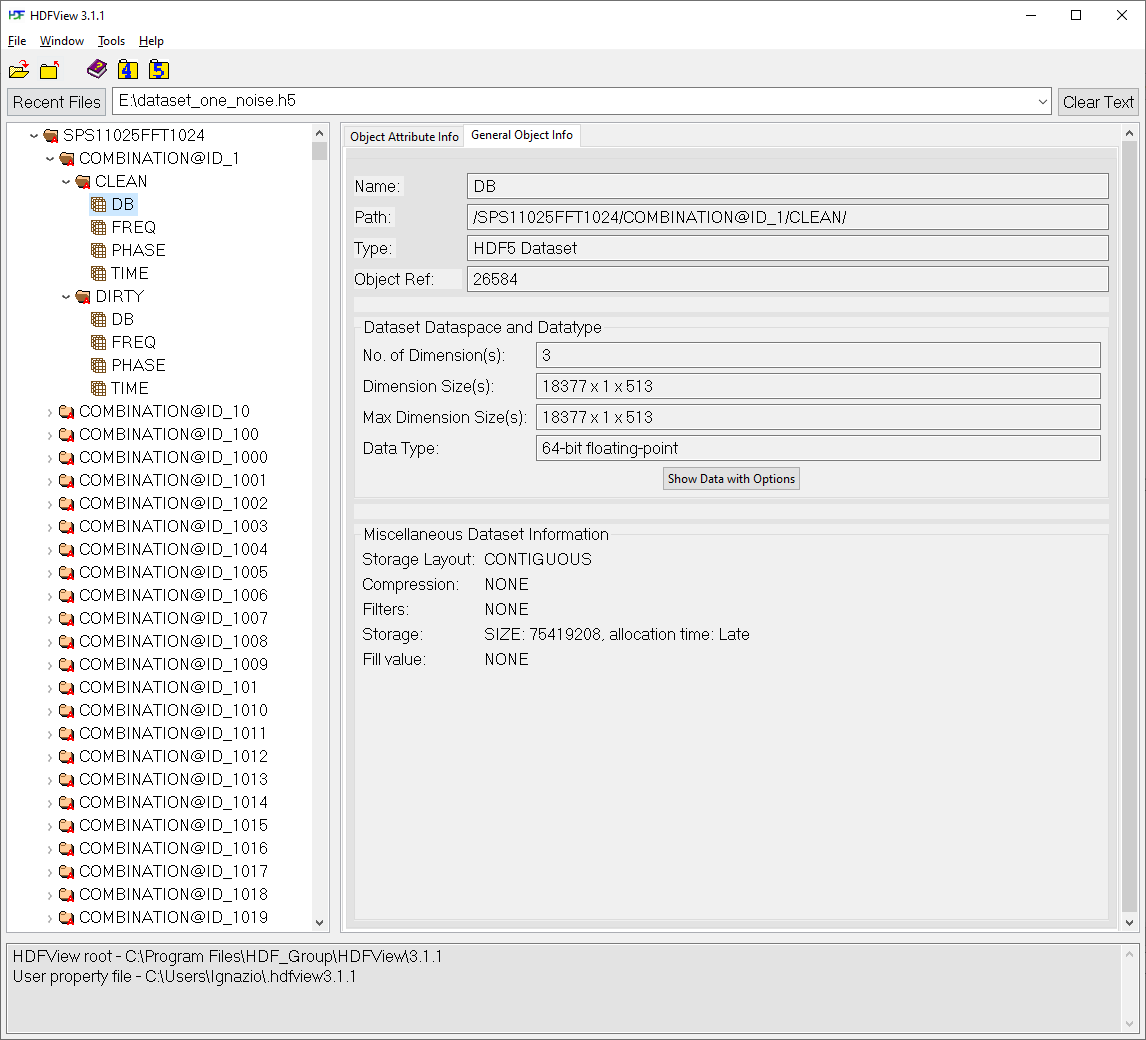
\includegraphics[width=0.75\columnwidth]{../figures/HDF5_struct2}
		\caption{Estructura de los datos almacenados en el archivo HDF5}
		\label{fig: hdf5_struct2}
	\end{figure}
\end{frame}
		\subsection{Modelo de capas LSTM}
			\begin{frame}{Diseño e implementación de modelos.\newline Modelo de capas LSTM I}
	\vspace*{10pt}
	\normalsize{\underline{\textbf{Tipos de arquitectura}}}
	\vspace*{3pt}
	\begin{itemize}
		\scriptsize
		\item \textbf{One to one}\arrowTikz{0}clasificación de imágenes, una entrada (matriz de la imagen), una salida, la categoría.
		\item \textbf{One to many}\arrowTikz{0}generación de títulos para imágenes, una entrada (matriz de la imagen), varias salidas, las diferentes palabras.
		\item \textbf{Many to one}\arrowTikz{0}análisis de sentimiento, entran varias palabras, se clasifica como positiva o negativa.
		\item \textbf{Many to many}\arrowTikz{0}traducción de texto, varias palabras en un idioma a la entrada y varias a la salida en otro idioma.
		\item \textbf{Many to many}\arrowTikz{0}entradas y salidas sincronizadas, clasificación de vídeo.
	\end{itemize}
	\vspace*{-10pt}
	\begin{figure}[ht!]
		\centering
		\resizebox{\textwidth}{!}{
			\begin{tikzpicture}
			\tikzstyle{input} = [draw,inner sep=7,minimum size=10, draw=black, fill=red!20, text width=20, text centered,rotate=90]
			\tikzstyle{hidden} = [draw,inner sep=7,minimum size=10, draw=black, fill=green!20, text width=20, text centered,rotate=90]
			\tikzstyle{output} = [draw,inner sep=7,minimum size=10, draw=black, fill=blue!20, text width=20, text centered,rotate=90]
			\tikzstyle{invisible} = [outer sep=0,inner sep=0,minimum size=0]
			\tikzstyle{stealth} = [-stealth, very thick]
			\fill [rounded corners, fill=gray!10] (-4,3.5) rectangle (-3,-2.5);
			\fill [rounded corners, fill=gray!10] (-2.5,3.5) rectangle (0.5,-2.5);
			\fill [rounded corners, fill=gray!10] (1,3.5) rectangle (4,-2.5);
			\fill [rounded corners, fill=gray!10] (4.5,3.5) rectangle (9.5,-2.5);
			\fill [rounded corners, fill=gray!10] (10,3.5) rectangle (13,-2.5);
			\node [input] (v1) at (-3.5,-1.5) {};
			\node [hidden] (v2) at (-3.5,0.5) {};
			\node [output] (v3) at (-3.5,2.5) {};
			\node [input] (v4) at (-2,-1.5) {};
			\node [hidden] (v5) at (-2,0.5) {};
			\node [hidden] (v7) at (-1,0.5) {};
			\node [hidden] (v8) at (0,0.5) {};
			\node [output] (v6) at (-2,2.5) {};
			\node [output] (v9) at (-1,2.5) {};
			\node [output] (v10) at (0,2.5) {};
			\node [input] (v11) at (1.5,-1.5) {};
			\node [input] (v13) at (2.5,-1.5) {};
			\node [input] (v15) at (3.5,-1.5) {};
			\node [hidden] (v12) at (1.5,0.5) {};
			\node [hidden] (v14) at (2.5,0.5) {};
			\node [hidden] (v16) at (3.5,0.5) {};
			\node [output] (v17) at (3.5,2.5) {};
			\node [input] (v18) at (5,-1.5) {};
			\node [input] (v20) at (6,-1.5) {};
			\node [input] (v22) at (7,-1.5) {};
			\node [hidden] (v19) at (5,0.5) {};
			\node [hidden] (v21) at (6,0.5) {};
			\node [hidden] (v23) at (7,0.5) {};
			\node [hidden] (v25) at (8,0.5) {};
			\node [hidden] (v27) at (9,0.5) {};
			\node [output] (v24) at (7,2.5) {};
			\node [output] (v26) at (8,2.5) {};
			\node [output] (v28) at (9,2.5) {};
			\node [input] (v29) at (10.5,-1.5) {};
			\node [input] (v32) at (11.5,-1.5) {};
			\node [input] (v35) at (12.5,-1.5) {};
			\node [hidden] (v30) at (10.5,0.5) {};
			\node [hidden] (v33) at (11.5,0.5) {};
			\node [hidden] (v36) at (12.5,0.5) {};
			\node [output] (v31) at (10.5,2.5) {};
			\node [output] (v34) at (11.5,2.5) {};
			\node [output] (v37) at (12.5,2.5) {};
			\draw [stealth] (v1) edge (v2);
			\draw [stealth] (v2) edge (v3);
			\draw [stealth] (v4) edge (v5);
			\draw [stealth] (v5) edge (v6);
			\draw [stealth] (v5) edge (v7);
			\draw [stealth] (v7) edge (v8);
			\draw [stealth] (v7) edge (v9);
			\draw [stealth] (v8) edge (v10);
			\draw [stealth] (v11) edge (v12);
			\draw [stealth] (v13) edge (v14);
			\draw [stealth] (v15) edge (v16);
			\draw [stealth] (v12) edge (v14);
			\draw [stealth] (v14) edge (v16);
			\draw [stealth] (v16) edge (v17);
			\draw [stealth] (v18) edge (v19);
			\draw [stealth] (v20) edge (v21);
			\draw [stealth] (v22) edge (v23);
			\draw [stealth] (v23) edge (v24);
			\draw [stealth] (v25) edge (v26);
			\draw [stealth] (v27) edge (v28);
			\draw [stealth] (v19) edge (v21);
			\draw [stealth] (v21) edge (v23);
			\draw [stealth] (v23) edge (v25);
			\draw [stealth] (v25) edge (v27);
			\draw [stealth] (v29) edge (v30);
			\draw [stealth] (v30) edge (v31);
			\draw [stealth] (v32) edge (v33);
			\draw [stealth] (v33) edge (v34);
			\draw [stealth] (v35) edge (v36);
			\draw [stealth] (v36) edge (v37);
			\draw [stealth] (v30) edge (v33);
			\draw [stealth] (v33) edge (v36);
			
			\node [invisible] at (-3.5,4) {One to one};
			\node [invisible] at (-1,4) {One to many};
			\node [invisible] at (2.5,4) {Many to one};
			\node [invisible] at (7,4) {Many to many};
			\node [invisible] at (11.5,4) {Many to many};
			\node [invisible] at (-5.5,-1.5) {input layer};
			\node [invisible] at (-5.5,0.5) {hidden layer};
			\node [invisible] at (-5.5,2.5) {Output layer};
			\end{tikzpicture}
		}      
		\caption{Arquitecturas de modelo}%\cite{karpathy}.
		\label{fig: model_archs}
	\end{figure}
\end{frame}
\begin{frame}[fragile]{Diseño e implementación de modelos.\newline Modelo de capas LSTM II}
\begin{lstlisting}[basicstyle=\tiny\ttfamily, caption={Resumen del modelo},captionpos=b, label={lst: model_resume},frame=none, xleftmargin=.2\textwidth]
_________________________________________________________________
Layer (type)                 Output Shape              Param #   
=================================================================
lstm (LSTM)                  (None, 1, 512)            1562624   
_________________________________________________________________
lstm_1 (LSTM)                (None, 1, 512)            2099200   
_________________________________________________________________
lstm_2 (LSTM)                (None, 512)               2099200   
_________________________________________________________________
dense (Dense)                (None, 250)               128250    
=================================================================
Total params: 5,889,274
Trainable params: 5,889,274
Non-trainable params: 0
_________________________________________________________________
\end{lstlisting}
\end{frame}
\begin{frame}[fragile]{Diseño e implementación de modelos.\newline Modelo de capas LSTM III}
	\vspace*{5pt}
	Debido al gran número de datos, \textbf{294 Gbytes}, se debe entrenar con un generador de secuencias, además los datos van a ser normalizados
	\begin{figure}
		\centering
		\begin{subfigure}[t]{0.4\textwidth}
			\centering
			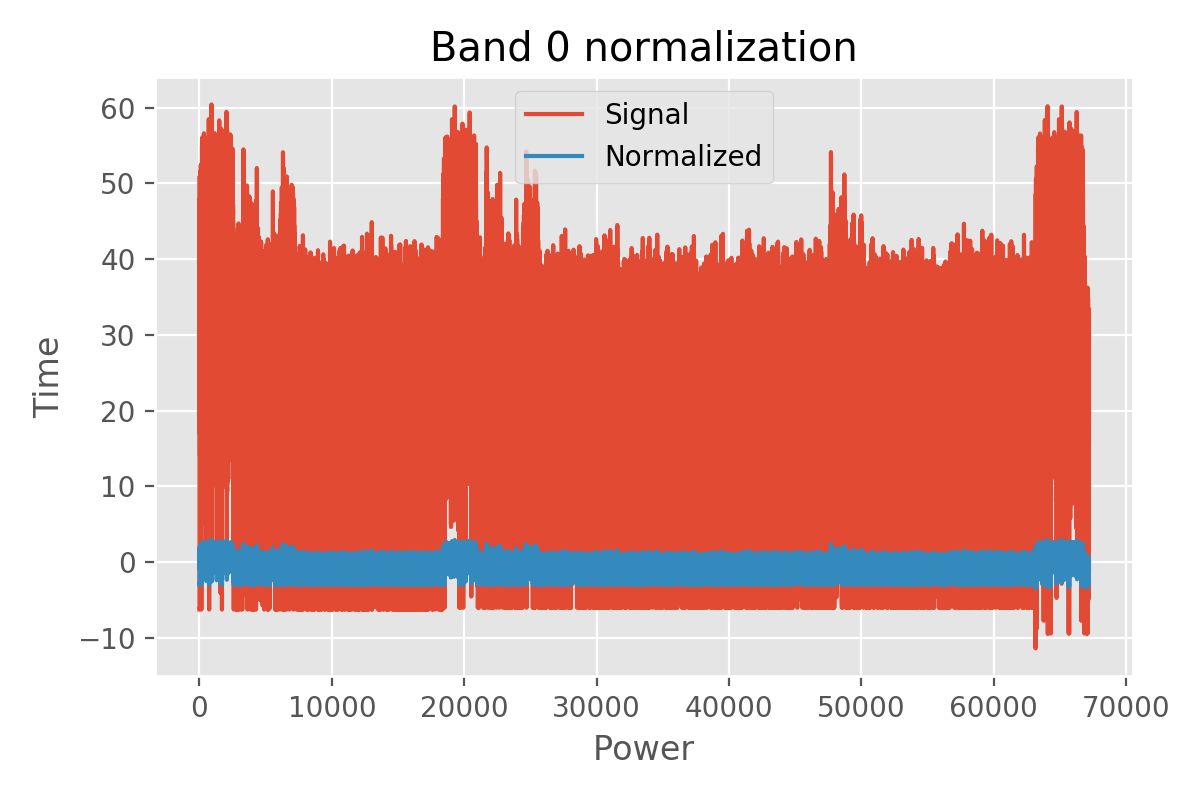
\includegraphics[width=\columnwidth]{../figures/band0_norm}
			\vspace*{-7pt}
			\caption{Comparación de la señal con su normalización en tiempo para la banda cero de un mismo audio con ruido}
			\label{fig: norm_time}
		\end{subfigure}%
		\hspace*{10pt}
		\begin{subfigure}[t]{0.4\textwidth}
			\centering
			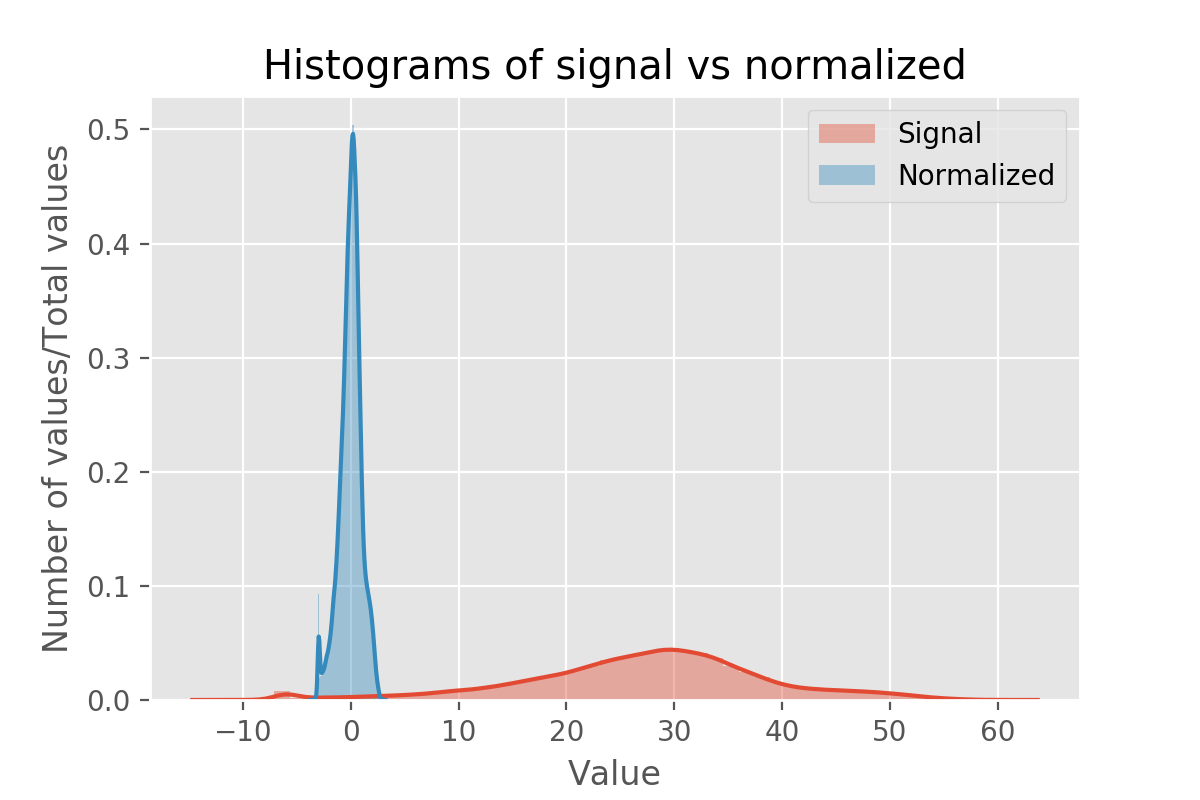
\includegraphics[width=\columnwidth]{../figures/band0_norm_hist}
			\vspace*{-7pt}
			\caption{Comparación de los histogramas de la señal y su normalización para la banda cero de un mismo audio con ruido}
			\label{fig: norm_hist}
		\end{subfigure}
	\end{figure}
	\vspace*{-17pt}
	\begin{figure}
		\centering
		\begin{subfigure}[t]{0.4\textwidth}
			\centering
			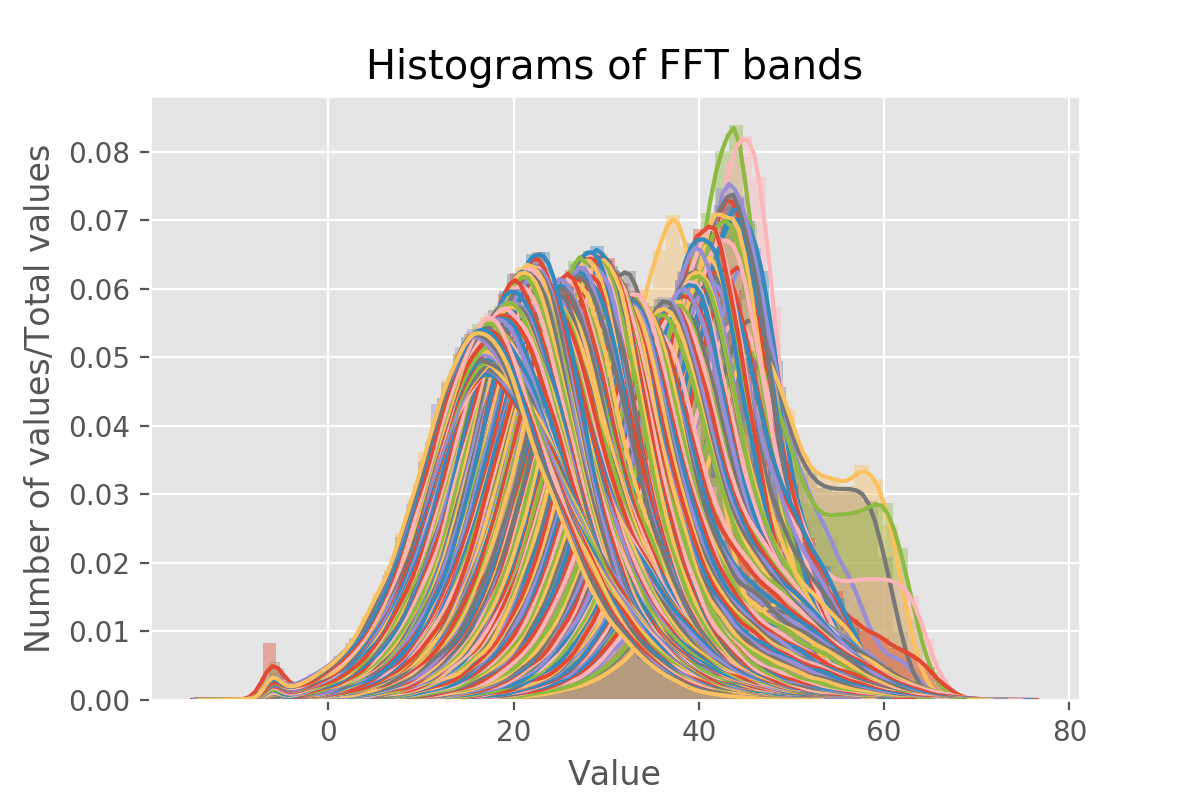
\includegraphics[width=\textwidth]{../figures/bands_hist}
			\vspace*{-7pt}
			\caption{Histograma de todas las bandas}
			\label{fig: bands_hist}
		\end{subfigure}%
		\hspace*{10pt}
		\begin{subfigure}[t]{0.4\textwidth}
			\centering
			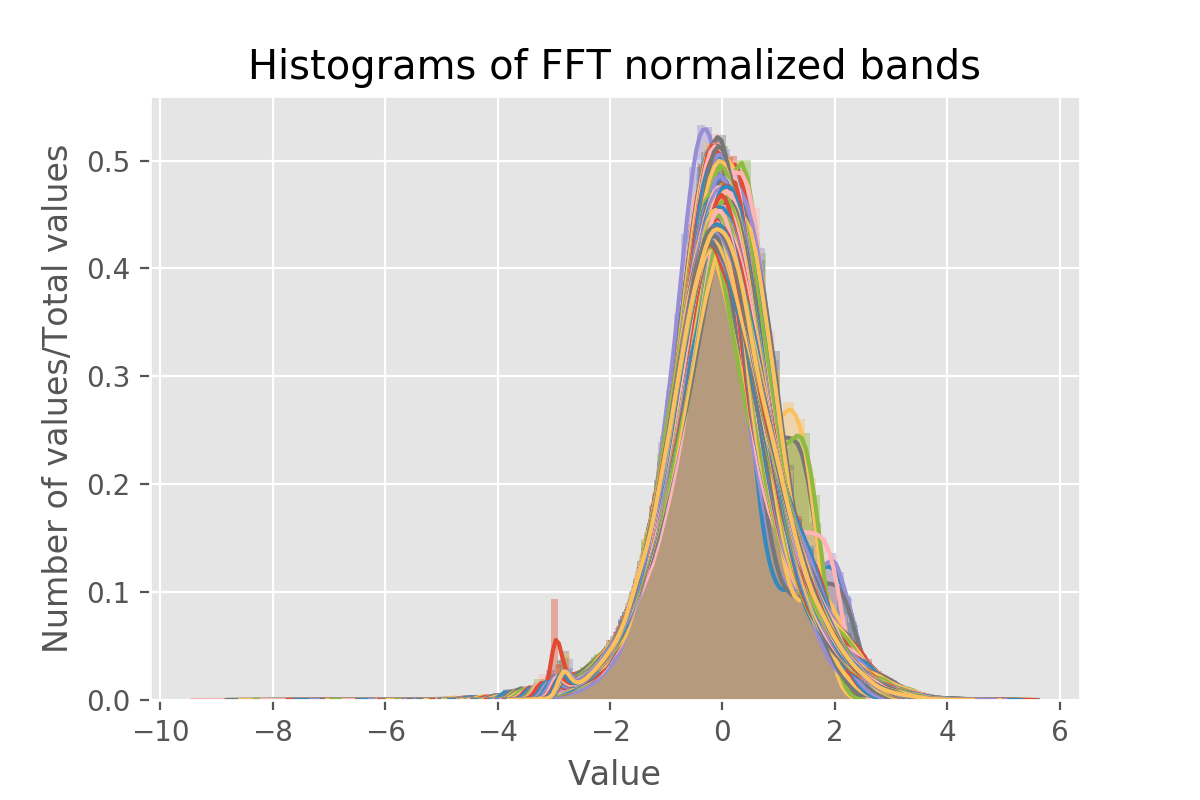
\includegraphics[width=\textwidth]{../figures/bands_norm_hist}
			\vspace*{-7pt}
			\caption{Histograma de todas las bandas normallizadas}
			\label{fig: bands_norm_hist}
		\end{subfigure}
	\end{figure}
\end{frame}
	% RESULTS
	\section{Análisis de los resultados obtenidos}
		\chapter{Conclusiones y planes de mejora}
\lipsum[3-6]
	% CONCLUSIONS
	\section{Conclusiones y propuestas de mejora}
		\chapter{Conclusiones y planes de mejora}
\lipsum[3-6]
	
	% THANKS PAGE
	\bgroup
%\setbeamercolor{background canvas}{bg=beamer@headercolor}
\usebackgroundtemplate{}
\begin{frame}[plain,noframenumbering]{}
	\begin{minipage}[t]{\linewidth-2\fboxsep-2\fboxrule}
		\centering
		\vspace{-0.329\paperheight}
		\hspace*{-1.133\paperwidth}
		\tikzGraphic
	\end{minipage}
	\hspace*{-1.15\SidebarWidth}
	\centering
	\huge
	\ \textcolor{white}{GRACIAS POR SU}
	%\vspace{1 cm}
	\\
	\hspace*{-1.15\SidebarWidth} 
	\textcolor{white}{ATENCIÓN}
	\\
	\vspace*{1 cm}
	\hspace*{-1.15\SidebarWidth}
	%\textcolor{white}{ifinazzi@gte.esi.us.es}
	\vspace*{-2 cm}
\end{frame}
\egroup
\end{document}